\documentclass[11pt,a4paper]{article}

% ── Encodage et langue ───────────────────────────────────────────────────────
\usepackage[utf8]{inputenc}
\usepackage[T1]{fontenc}
\usepackage[english]{babel}

% ── Mise en page ─────────────────────────────────────────────────────────────
\usepackage[margin=2.5cm]{geometry}
\usepackage{setspace}
\onehalfspacing

% ── Packages scientifiques ───────────────────────────────────────────────────
\usepackage{amsmath,amssymb}
\usepackage{graphicx}
\usepackage{booktabs}
\usepackage{longtable}
\usepackage{multirow}
\usepackage{xcolor}
\usepackage{placeins}
\usepackage{hyperref}
\hypersetup{
    colorlinks=true,
    linkcolor=blue!60!black,
    citecolor=green!50!black,
    urlcolor=blue!70!black
}

% ── Bibliographie ────────────────────────────────────────────────────────────
\usepackage[numbers,sort&compress]{natbib}

% ── Commandes personnalisées ─────────────────────────────────────────────────
\newcommand{\mtb}{\textit{Mycobacterium tuberculosis}}
\newcommand{\spdi}[1]{\texttt{#1}}
\newcommand{\lignee}[1]{\textsf{#1}}
% \newcommand{\todo}[1]{\textcolor{red}{\textbf{[TODO: #1]}}}  % removed for submission

% ══════════════════════════════════════════════════════════════════════════════
\title{Convergent evolution toward drug resistance and immune evasion in
       \mtb{} lineage L4.11: phylogenomic characterisation of two novel
       sub-lineages from Bangladesh and Peru}

\author{Christophe Guyeux\textsuperscript{1,*}
  \and Cl\'ement Lecarpentier\textsuperscript{1}
  \and Guislaine Refr\'egier\textsuperscript{2}
  \and Christophe Sola\textsuperscript{2}
  \\[6pt]
  {\normalsize\textsuperscript{1}FEMTO-ST Institute, DISC Department, Univ.\ Bourgogne Franche-Comt\'e, Besan\c{c}on, France}\\
  {\normalsize\textsuperscript{2}Universit\'e Paris-Saclay, CNRS, AgroParisTech, I2BC, Orsay, France}\\
  {\normalsize\textsuperscript{*}Corresponding author: \texttt{christophe.guyeux@univ-fcomte.fr}}
}

\date{\today}

% ══════════════════════════════════════════════════════════════════════════════
\begin{document}
\maketitle

% ── Abstract ─────────────────────────────────────────────────────────────────
\begin{abstract}
	Lineage~4 of \mtb{} is the most geographically widespread lineage of the
	\mtb{} complex.  Among its sub-lineages, \lignee{L4.11} (within
	Coll~\lignee{4.9} / Stucki~\lignee{4.10}) remains poorly characterised.
	Using 825 whole-genome sequences from the TBannotator~v3.2 database, we
	performed a comprehensive phylogenomic analysis combining marker-based
	lineage definition, drug resistance profiling, structural variation,
	selection pressure analysis, transmission clustering, and molecular dating.

	We identified 8~core-exclusive SPDIs defining \lignee{L4.11} and two
	novel sub-lineages --- \lignee{L4.11.1} (91~SRAs, predominantly
	Bangladesh, 86\% MDR) and \lignee{L4.11.2} (731~SRAs, predominantly
	Peru, 27\% MDR) --- with sharply contrasting resistance profiles.
	\lignee{L4.11.1} carries near-universal \textit{katG}~S315T (91\%),
	while \lignee{L4.11.2} harbours the \textit{mmpR5}~Ile67fs
	bedaquiline resistance-associated variant (24\%), paradoxically silenced
	by an epistatic \textit{mmpL5} frameshift.
	Both sub-lineages carry high IS6110 copy numbers (median~10),
	with insertions disrupting the DosR dormancy regulon.  Lineage-fixed
	cell-envelope mutations define a remodelled lipid programme.
	Convergent evolution analysis identifies 106~homoplastic sites with
	elevated $p_N/p_S$ ratios (2.00~overall), concentrated in PE/PPE
	and cell-wall genes.  Transmission clustering (12-SNP threshold, 27\%
	overall) is significantly higher in \lignee{L4.11.2} (29\%) than
	\lignee{L4.11.1} (10\%).  Molecular clock analysis estimates the
	TMRCA around 1965 (bootstrap 95\% CI: 1560--1996), although weak
	temporal signal ($R^2 = 0.008$) warrants caution.
	Several features --- IS6110 expansion, \textit{rpoC} compensatory
	mutations, PE/PPE diversification --- parallel the Beijing lineage (L2),
	suggesting convergent evolutionary strategies toward drug resistance
	and immune evasion from different genetic backgrounds.
\end{abstract}

\noindent\textbf{Keywords:} \mtb, phylogenomics, convergent evolution, drug resistance,
bedaquiline, IS6110, transmission clustering, PE/PPE, Bangladesh, Peru

% ── Introduction ─────────────────────────────────────────────────────────────
\section{Introduction}

Tuberculosis (TB) remains one of the leading causes of death from a single
infectious agent worldwide, with an estimated 10.8~million incident cases and
1.25~million deaths in 2023~\cite{who2024}.  The disease is caused by bacteria
of the \mtb{} complex (MTBC), a group of closely related obligate pathogens~\cite{sreevatsan1997,brites2015}
whose genetic diversity is organised into distinct phylogenetic lineages~\cite{comas2013}.
Understanding this diversity is critical for epidemiological surveillance,
drug resistance monitoring~\cite{sahal2023}, and the design of targeted interventions.

Among the ten recognised human-adapted lineages (L1--L10)~\cite{guyeux2024}, \mtb{} lineage~4
(Euro-American) is the most geographically widespread, occurring at significant
frequencies across all inhabited continents~\cite{stucki2016}.  It also displays
the greatest internal genetic diversity, with at least ten major sub-lineages
identified to date.  Population genomic analyses have revealed that lineage~4
comprises both ``generalist'' sub-lineages --- globally distributed and
characterised by a higher proportion of variable T-cell epitopes --- and
``specialist'' sub-lineages with more restricted geographic
ranges~\cite{stucki2016}.

Several classification systems have been proposed to capture this diversity.
Coll~et~al.~\cite{coll2014} defined the first widely adopted 62-SNP
barcode, identifying sub-lineages up to \lignee{4.9}.  Stucki~et~al.~\cite{stucki2016}
subsequently characterised ten sub-lineages (L4.1--L4.10) using genome-wide
variation and principal component analysis, showing that \lignee{L4.10/PGG3}
accounts for 11.9\% of lineage~4 isolates globally and is detected in
47~countries, consistent with a generalist profile.
Napier~et~al.~\cite{napier2020} further expanded the barcode to 90~SNPs
covering 90~(sub-)lineages, Later Netikul \textit{et al.} and Thawornwattana \textit{et al.} improved the designation and barcode of L1 and L2 respectively ~\cite{netikul2022,thawornwattana2021}, while Shitikov~et~al.
had contributed markers for the East Asian lineage (L2) and partially overlapping L4 groups ~\cite{shitikov2017}. 

The most comprehensive hierarchical framework to date was proposed by
Freschi~et~al.~\cite{freschi2021}, who analysed 12\,170 genomes and defined
69~sub-lineages and 26~additional internal groups, including three new
sub-lineages within lineage~4 (4.11--4.13).  Their system employs an
``\texttt{i}'' suffix to denote internal groups within a sub-lineage,
e.g.\ \lignee{4.10.i2} designates an internal group of
Stucki's \lignee{4.10}.

The sub-lineage that is the focus of the present work, henceforth referred
to as \lignee{L4.11} following our nomenclature~\cite{senelle2023}, falls
within the scope of several existing classifications but is not resolved
as a distinct entity by any of them.
Table~\ref{tab:nomenclature} summarises how the five major
classification systems map to the \lignee{L4.11} clade.
Crucially, the Freschi designation ``\lignee{4.11}'' (defined by the SNP
at position 801\,008, coordinates on H37Rv NC000962.3) corresponds to our \lignee{L4.11.2}
sub-lineage (731/825~SRAs), not to the full \lignee{L4.11} clade.
The broader Freschi designation ``\lignee{4.10.i2}'' corresponds to a
separate clade centred on H37Rv (Guyeux~L4.9), not to our \lignee{L4.11}.
Our \lignee{L4.11} clade, defined by the SNP at position 13\,073, has no
exact equivalent in the Freschi system.  We retain the ``\lignee{L4.11}''
designation from our nomenclature~\cite{senelle2023} because it reflects
the first identification of this clade as a distinct phylogenetic unit;
the ``L'' prefix unambiguously distinguishes it from the Freschi numbering
(see Table~\ref{tab:nomenclature}).
Despite appearing in multiple nomenclature systems at coarser resolution,
the internal phylogenetic structure of this lineage has never been
explored in detail.

\begin{table}[htbp!]
	\centering
	\small
	\caption{Correspondence between classification systems for
		the clade studied here (\lignee{L4.11}, Guyeux nomenclature).
		$\supset$: the system designation is broader than \lignee{L4.11}
		(our clade is a subset).
		$\subset$: the system designation is narrower
		(a sub-group within our \lignee{L4.11}).}
	\label{tab:nomenclature}
	\begin{tabular}{lccl}
		\toprule
		\textbf{System} & \textbf{Designation} & \textbf{Relation} & \textbf{Scope} \\
		\midrule
		\textbf{This study} & \lignee{L4.11} & --- & Target clade (825~SRAs) \\
		Coll~et~al.~(2014)~\cite{coll2014} & \lignee{4.9} & $\supset$ & Broader; includes other sub-lineages \\
		Stucki~et~al.~(2016)~\cite{stucki2016} & \lignee{4.10} & $\supset$ & Broader; generalist clade \\
		Freschi~et~al.~(2021)~\cite{freschi2021} & \lignee{4.10.i2} & $\neq$ & Separate clade (H37Rv/L4.9) \\
		Freschi~et~al.~(2021)~\cite{freschi2021} & \lignee{4.11} & $\subset$ & Matches our \lignee{L4.11.2} (731/825) \\
		Napier~et~al.~(2020)~\cite{napier2020} & \lignee{4/4.9} & $\supset$ & Broader; insufficient resolution \\
		Shitikov~et~al.~(2017)~\cite{shitikov2017} & \lignee{4/4.9} & $\supset$ & Broader; insufficient resolution \\
		\bottomrule
	\end{tabular}
\end{table}

Circumstantial evidence suggests clinical relevance.  Vargas~et~al.~\cite{vargas2023}
recently investigated the role of epistasia in drug-resistance among 31,000 MTB complex genomes among which many belonging to Freschi sub-lineage~4.11 (i.e.\
a sub-group of our \lignee{L4.11}) and identified a monophyletic cluster
from Lima, Peru (1997--2012) harbouring co-occurring frameshift mutations in
\textit{mmpR5}(Rv0678) and \textit{mmpL5}. \textit{mmpR5} frameshift mutations are known to confer cross-resistance to
bedaquiline and clofazimine, two drugs increasingly used against
multidrug-resistant TB\@, by loss of function of mmpR5 (regulator) and constitutive overexpression of the efflux pump --- , however epistatic mutations on mmpL5 and mmpS5 may for some lineages restore an hypersusceptible phenotype (e.g in subgroups
of lineages 1.1.1.1 and 4.6) ~\cite{merker2020}. This finding underscores the need for a fine-grained understanding of taxonomic assignment of isolates in particular of \lignee{L4.11}'s internal structure to contextualise such resistance events.

In this work, we perform the first comprehensive phylogenomic analysis of
\lignee{L4.11} using 825~publicly available whole-genome sequences from the
TBannotator~v3.2 database.  Our objectives are:
(1)~to reconstruct the maximum-likelihood phylogeny and identify core-exclusive
SNPs that unambiguously define this lineage;
(2)~to assess the existence of novel sub-lineages not captured by current
classification systems;
(3)~to characterize the drug resistance landscape, including genotypic MDR and
pre-XDR profiles;
(4)~to analyse genomic structural variation, including IS6110 copy-number
expansion, gene deletions, and RD-typing;
(5)~to evaluate convergent evolution and selection pressures through homoplasy
detection and $p_N/p_S$ analysis;
(6)~to estimate transmission clustering rates within and between sub-lineages; and
(7)~to reconstruct the spatio-temporal history of this lineage through molecular clock analysis and ancestral geographic inference.


% ── Materials and Methods ────────────────────────────────────────────────────
\section{Materials and Methods}
\label{sec:methods}

% ─── 2.1 Data acquisition and quality control ────────────────────────────────
\subsection{Data acquisition and quality control}

\subsubsection{Genome selection and description of the TBannotator platform}

All analyses were conducted using TBannotator~v3.2~\cite{guyeux2024tbannotator,senelle2023},
an interactive phylogenomic analysis platform for \mtb  containing 274,800 SRAs extracted from the NCBI at the time of writing.
TBannotator provides an automated bioinformatics pipeline that retrieves
raw sequencing data from the NCBI Sequence Read Archive (SRA), performs
quality control with fastp~\cite{chen2018}, maps reads to the H37Rv reference genome
(\spdi{NC\_000962.3}) using minimap2~\cite{li2018}, calls variants with freebayes~\cite{garrison2012}, and
normalises them into SPDI notation  	\cite{mcinerney2004}
.
The platform maintains a curated database of variant profiles for all
publicly available MTBC genomes, enabling tree-aware interactive clade
exploration, marker discovery (core, core-exclusive, and near-exclusive
SPDIs), and cross-referencing with existing nomenclature systems.
Additionally, TBannotator records TBProfiler for RIF, INH, PZA and EMB drug-resistance prediction ~\cite{phelan2019} and allows easy extraction in a strain report, as assessed in an independent study ~\cite{auganova2025}.

All publicly available whole-genome sequences assigned to \lignee{L4.11} were
retrieved from the TBannotator~v3.2 database.
The lineage-defining marker \spdi{NC\_000962.3:1374351:C:T} was originally
identified from TBannotator~v2 through a two-step procedure: first, all
SRAs within a reasonable SPDI distance (i.e.\ number of variant
positions relative to H37Rv) from a central L4 strain in the Coll~4.9
neighbourhood were selected; second, a phylogenetic tree comprising these candidates together
with representatives of all other MTBC lineages was constructed, and the
core-exclusive marker shared by all SRAs of the resulting monophyletic
clade was identified.
Using this marker in the v3.2 database, a total of 847~candidate SRAs
were identified.
After phylogenetic reconstruction, 825~SRAs were confirmed as belonging to
the \lignee{L4.11} clade through interactive tree inspection; 22~candidates were
excluded as falling outside the L4.11 clade.
The 825-strain dataset originates from 57~BioProjects
(Table~\ref{tab:bioprojects}) and reflects the expanded catalogue of TBannotator~v3.2,
which approximately doubles the number of indexed genomes compared with
version~2.  Complete variant reports (annotated SNPs, gene coverage,
insertion sequences, and regions of difference) were retrieved for
all 825~SRAs via the TBannotator~v3.2 REST API.

For phylogenetic context, up to 10~SRAs per non-target lineage were included,
along with a \lignee{L8} outgroup (\spdi{SRR1173284}), the most
basal lineage of the MTBC sensu stricto.

\subsubsection{Sequencing quality assessment}

Prior to phylogenetic analysis, SRAs were filtered using three
quality-control criteria applied automatically by the TBannotator
pipeline: (i)~GC content between 61\% and 69\% (SRAs outside this
range indicate potential contamination or mixed infection);
(ii)~genome coverage $\geq$95\% of the H37Rv reference sequence; and
(iii)~mean sequencing depth $\geq$15$\times$.
SRAs failing any of these criteria were excluded from further analysis.

Mapping statistics for the 825~SRAs that passed QC were extracted
from TBannotator~v3.2 variant reports.  Mean sequencing depth
ranged from 20.8$\times$ to 462.0$\times$ (median 87.0$\times$).
Genome coverage exceeded 95\% in all SRAs.
The depth distribution was bimodal, with 46\% of SRAs in the
50--100$\times$ range and 46\% in the 100--200$\times$ range;
only 3~SRAs (0.7\%) had depth below 30$\times$ but all maintained
$>$95\% coverage.
Insert sizes (fastp peak) ranged from 35 to 466~bp (median 260~bp),
with no significant difference between sub-lineages
(\lignee{L4.11.1}: 269~bp; \lignee{L4.11.2}: 258~bp), indicating that
the sequencing library protocols do not introduce systematic biases
between the two geographic foci.

Per-BioProject comparison revealed that the \lignee{L4.11.1} SRAs,
predominantly from PRJEB38938 (Bangladesh), had a lower median depth
(65.3$\times$) than the \lignee{L4.11.2} SRAs from CRyPTIC projects
PRJEB40777 (123.9$\times$) and PRJEB31443 (113.4$\times$).  SRAs
from PRJNA595834 (TANDEM, Peru, Indonesia) and PRJEB26924 (Damien Foundation)
exhibited elevated missing-gene counts (median 42), consistent with the
biologically confirmed Rv1758--Rv1762c deletion rather than sequencing
artefacts.  No SRAs were excluded on the basis of sequencing quality.

% ─── 2.2 Variant representation and phylogenetics ────────────────────────────
\subsection{Variant representation and phylogenetics}

Variants were represented in SPDI notation~\cite{mcinerney2004},
enabling unambiguous identification across reference coordinates.

A binary presence/absence matrix (pan-SPDI) was constructed on all polymorphic markers and used as input
for maximum-likelihood inference with RAxML-NG~\cite{kozlov2019} under the
BIN+$\Gamma$ model. A similar analysis was performed on SNPs only using the GTR+$\Gamma$ (Gamma-Time Reversible) model, and very similar results were obtained (results not shown). The input alignment for the global tree reconstruction included 825~\lignee{L4.11}
SRAs plus up to 10~SRAs per non-target lineage and one outgroup (see Figure 1).
After removal of 70~exactly identical sequence pairs by RAxML-NG, the final
alignment comprised 68\,124~sites and 4\,818~informative patterns across
1\,095~taxa, for the
BIN+$\Gamma$  analysis.

For each clade of interest, we computed:
\begin{itemize}
	\item \textbf{Core SPDIs}: variants present in \emph{all} SRAs of the clade.
	\item \textbf{Core-exclusive SPDIs}: core variants absent from all SRAs
	      outside the clade.
\end{itemize}

Identified SNPs were cross-referenced against existing lineage-defining
markers from Coll, Freschi, Napier, Stucki, classification systems \cite{coll2014,freschi2021,napier2020,stucki2016}.

% ─── 2.3 Functional genomic analyses ─────────────────────────────────────────
\subsection{Functional genomic analyses}

\subsubsection{Drug resistance profiling}

Genotypic drug resistance predictions were derived from the annotated
SNPs in the TBannotator~v3.2 variant reports for all 825~SRAs.
Each SNP carries SnpEff functional annotation (gene, HGVS protein
change, impact class) \cite{cingolani2012}. resistance-associated mutations were identified
by cross-referencing with the WHO Catalogue of mutations associated
with drug resistance (2nd~edition, 2023;~\cite{who2023catalogue}).
A mutation was scored as resistance-conferring when the WHO grading
was ``R'' (associated with resistance) or ``F'' (associated with resistance ---
interim).  Resistance was systematically assessed for first-line drugs (isoniazid,
rifampicin, ethambutol, pyrazinamide) and for some key second-line drugs
including fluoroquinolones, streptomycin, bedaquiline, and clofazimine.
Multidrug resistance (MDR) was defined as resistance to
isoniazid and rifampicin.  Sub-lineage-specific resistance profiles
were compared using Fisher's exact test and odds ratios with 95\%
confidence intervals (Bonferroni-corrected).

\subsubsection{IS6110 copy-number estimation and gene content analysis}

Insertion sequence profiles were extracted from TBannotator~v3.2
variant reports for all 825~SRAs.  TBannotator detects IS insertion
positions by analysing soft-clipping signals in the BAM alignment:
reads whose clipped portion maps to a known IS element identify the
insertion site, orientation (forward or reverse), and element identity.
IS6110 copy numbers, novel insertion sites, and insertion orientations
were computed for all 825~SRAs (91~\lignee{L4.11.1},
731~\lignee{L4.11.2}, 3~basal).

Gene deletions were inferred from the variant reports
(825~SRAs), which record ``missing genes'' (genes with $<$5\%
coverage) associated to ``missing RD'' (those already named and new custom segments).  Deletions shared by $\geq$90\% of a
sub-lineage were considered as lineage-defining.

\subsubsection{In silico RD-typing and detection of new genomic structural variation}

Regions of difference (RD) were typed \textit{in silico} using the
\texttt{missing\_rd} and \texttt{large\_rd} fields of the TBannotator~v3.2
variant reports, which catalogue 4\,850~genomic segments screened per
strain, including both previously described RDs (RD715, DS5, DS13, RD3, ``149'',
\textit{etc.}) and custom segments identified by the pipeline designated as CUS \cite{bespiatykh2021}.
A segment was scored as deleted when its coverage fell below 5\%
of the genome-wide median.

\subsubsection{Virulence annotation and selection pressure}

Virulence-associated mutations were annotated by functional category:
PE/PPE family, \textit{mce} operons, ESX/Type~VII secretion, lipid
metabolism, regulatory systems (sigma factors, two-component systems),
and toxin--antitoxin systems.  Functional annotations were obtained from
Mycobrowser (mycobrowser.epfl.ch) and the literature.

Selection pressure was assessed using the site-based ratio of unique
non-synonymous to synonymous variant positions ($p_N/p_S$), computed across
all protein-coding genes with at least one variant in the 825-strain
dataset.  The $p_N/p_S$ ratio was calculated for each functional category
and compared between sub-lineages.
Because this site-based metric does not correct for the relative
number of non-synonymous and synonymous opportunities, it is inherently
biased upward in recently diverged, clonal populations such as
\mtb{}~\cite{rocha2006,kryazhimskiy2008}; values $>1$ should therefore
be interpreted as an excess of non-synonymous variants rather than
unequivocal evidence of positive selection.

% ─── 2.4 Epidemiological and evolutionary analyses ───────────────────────────
\subsection{Epidemiological and evolutionary analyses}

\subsubsection{Transmission clustering}

Pairwise genetic distances between all 825~SRAs were computed as the
symmetric difference of their SPDI variant sets.  Because all SRAs
were called against the same reference with an identical pipeline, this
measure is functionally equivalent to a core-genome SNP distance.
SRAs within $<$12~SNPs were defined as putative transmission clusters
using single-linkage clustering \cite{walker2013}.  Clustering rates were compared between
sub-lineages using Fisher's exact test.

\subsubsection{Homoplasy detection}

Homoplastic mutations (convergent evolution) were identified as SPDI
variants that arose independently on multiple branches of the Maximum likelihood (ML) tree.
Sites present in $\geq$3 SRAs from both sub-lineages but absent from
the common ancestor were flagged as candidate homoplasies.  Functional
enrichment of homoplastic sites was assessed by gene category.

% ─── 2.5 Molecular dating and ancestral reconstruction ──────────────────────
\subsection{Molecular dating and ancestral geographic reconstruction}

To estimate the time to the most recent common ancestor (TMRCA) of
\lignee{L4.11} and reconstruct ancestral geographic states, we used
TreeTime~v0.11.4~\cite{sagulenko2018}.  Of the 223~SRAs with known
collection dates, 143 were retained after removal of duplicates pruned
by RAxML-NG\@.  A root-to-tip regression was performed on these
143~SRAs (range: 2007--2025)
against the ML tree~\cite{zeineddine2023}.  Geographic ancestral reconstruction (mugration
analysis) was performed using the country of isolation for
591~SRAs (71.6\%) as a discrete trait under a GTR model.


% ── Results ──────────────────────────────────────────────────────────────────
\section{Results}

All analyses use the full set of 825~SRAs with complete
TBannotator~v3.2 variant reports (see Section~\ref{sec:methods}).

\subsection{Lineage definition and sub-lineage structure}

\begin{figure}[htbp!]
	\centering
	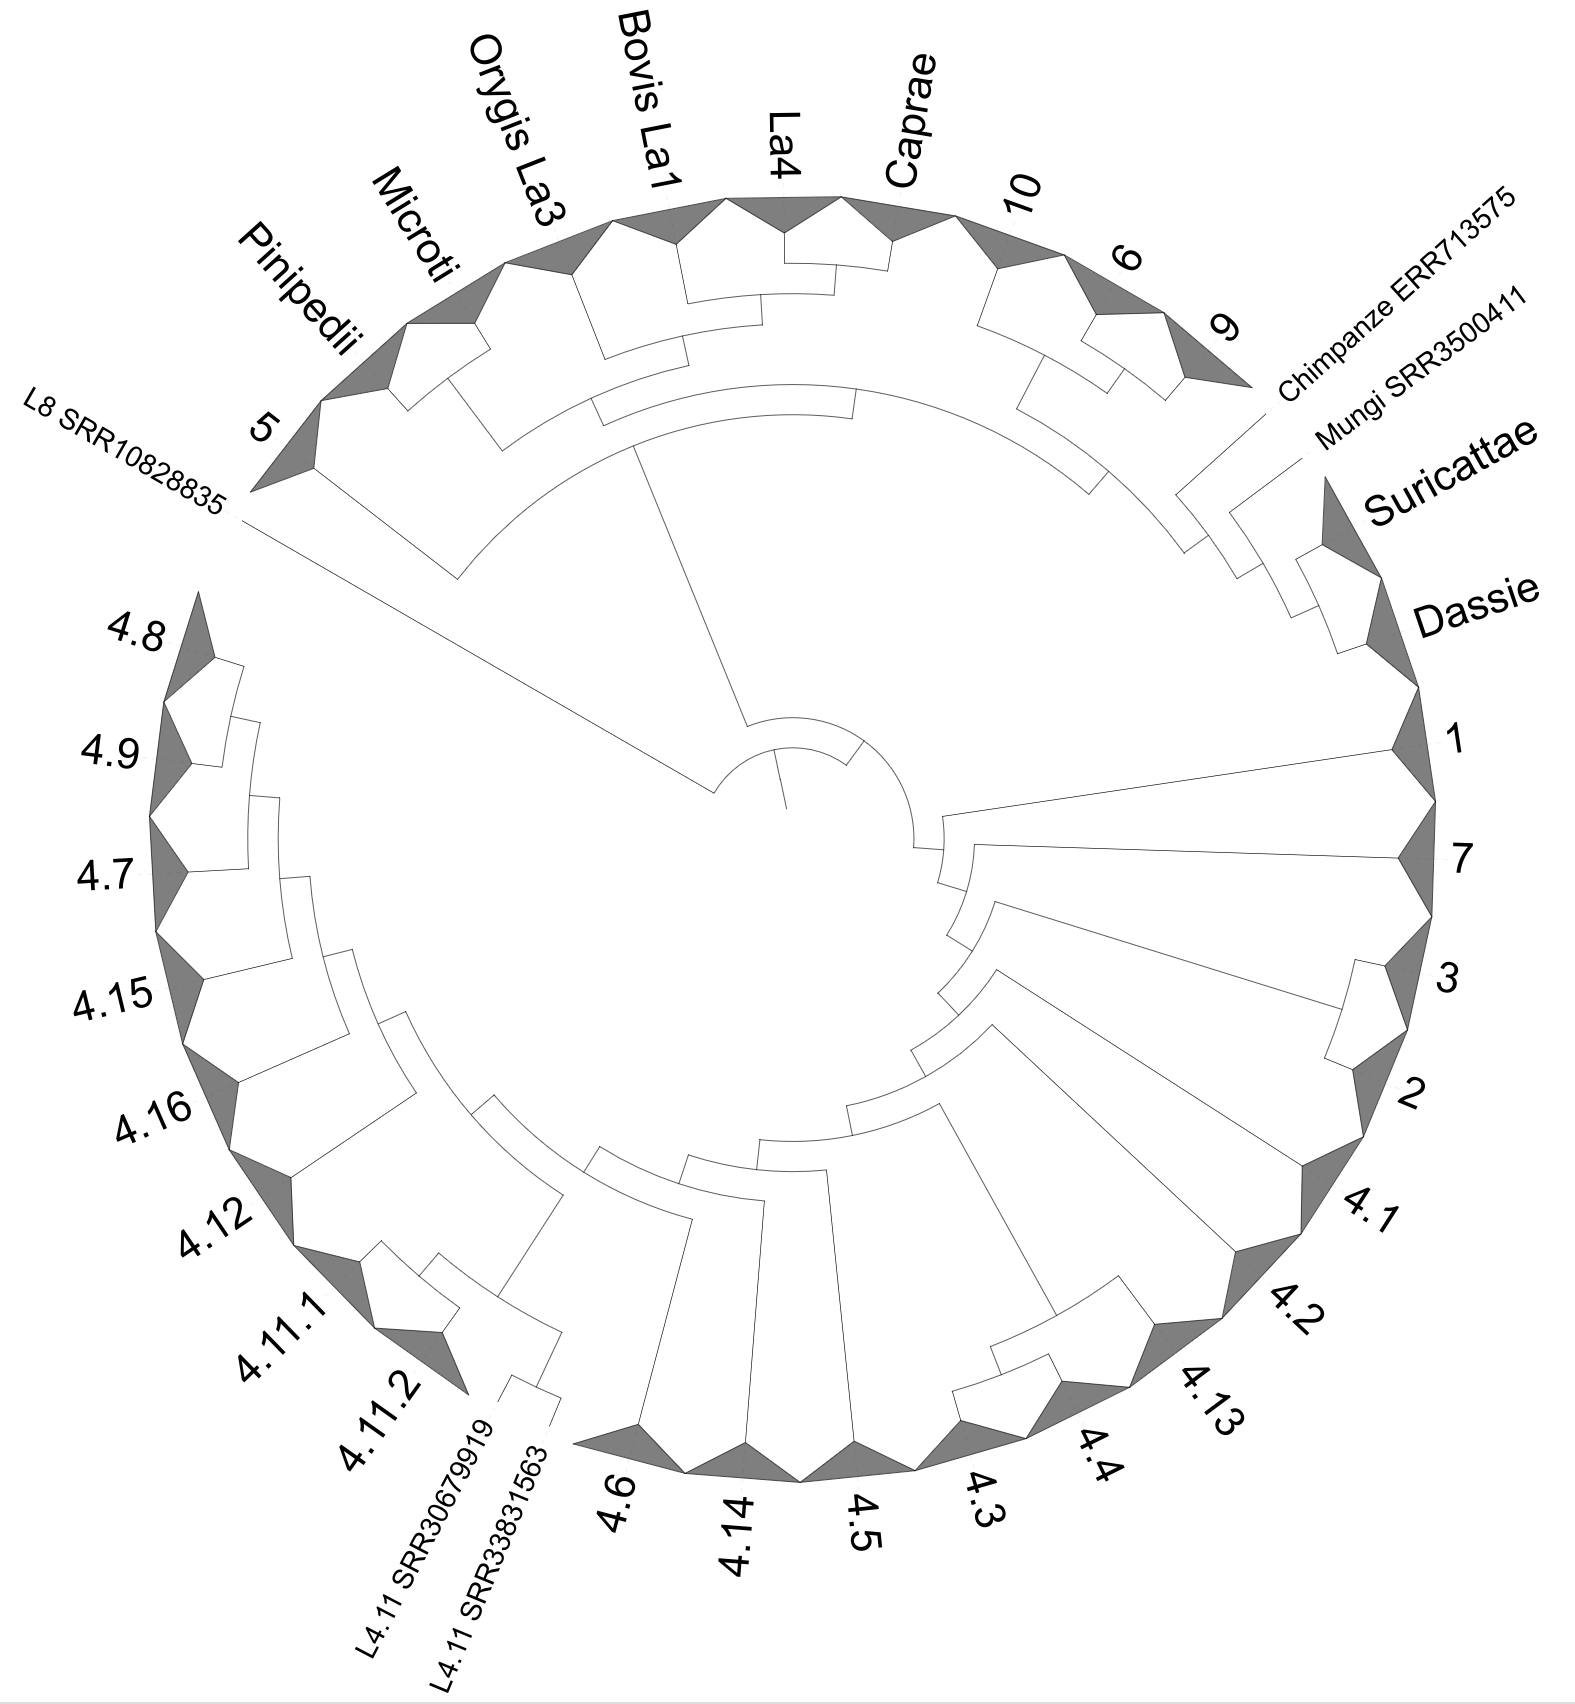
\includegraphics[width=0.6\textwidth]{figures/phylogenetic_view.png}
	\caption{Schematic position of \lignee{L4.11} within the Lineage~4 phylogeny.
		The two sub-lineages \lignee{L4.11.1} and \lignee{L4.11.2} are highlighted
		within the circular representation of the MTBC tree.}
	\label{fig:l4_phylogeny}
\end{figure}
\FloatBarrier

\begin{figure}[htbp!]
	\centering
	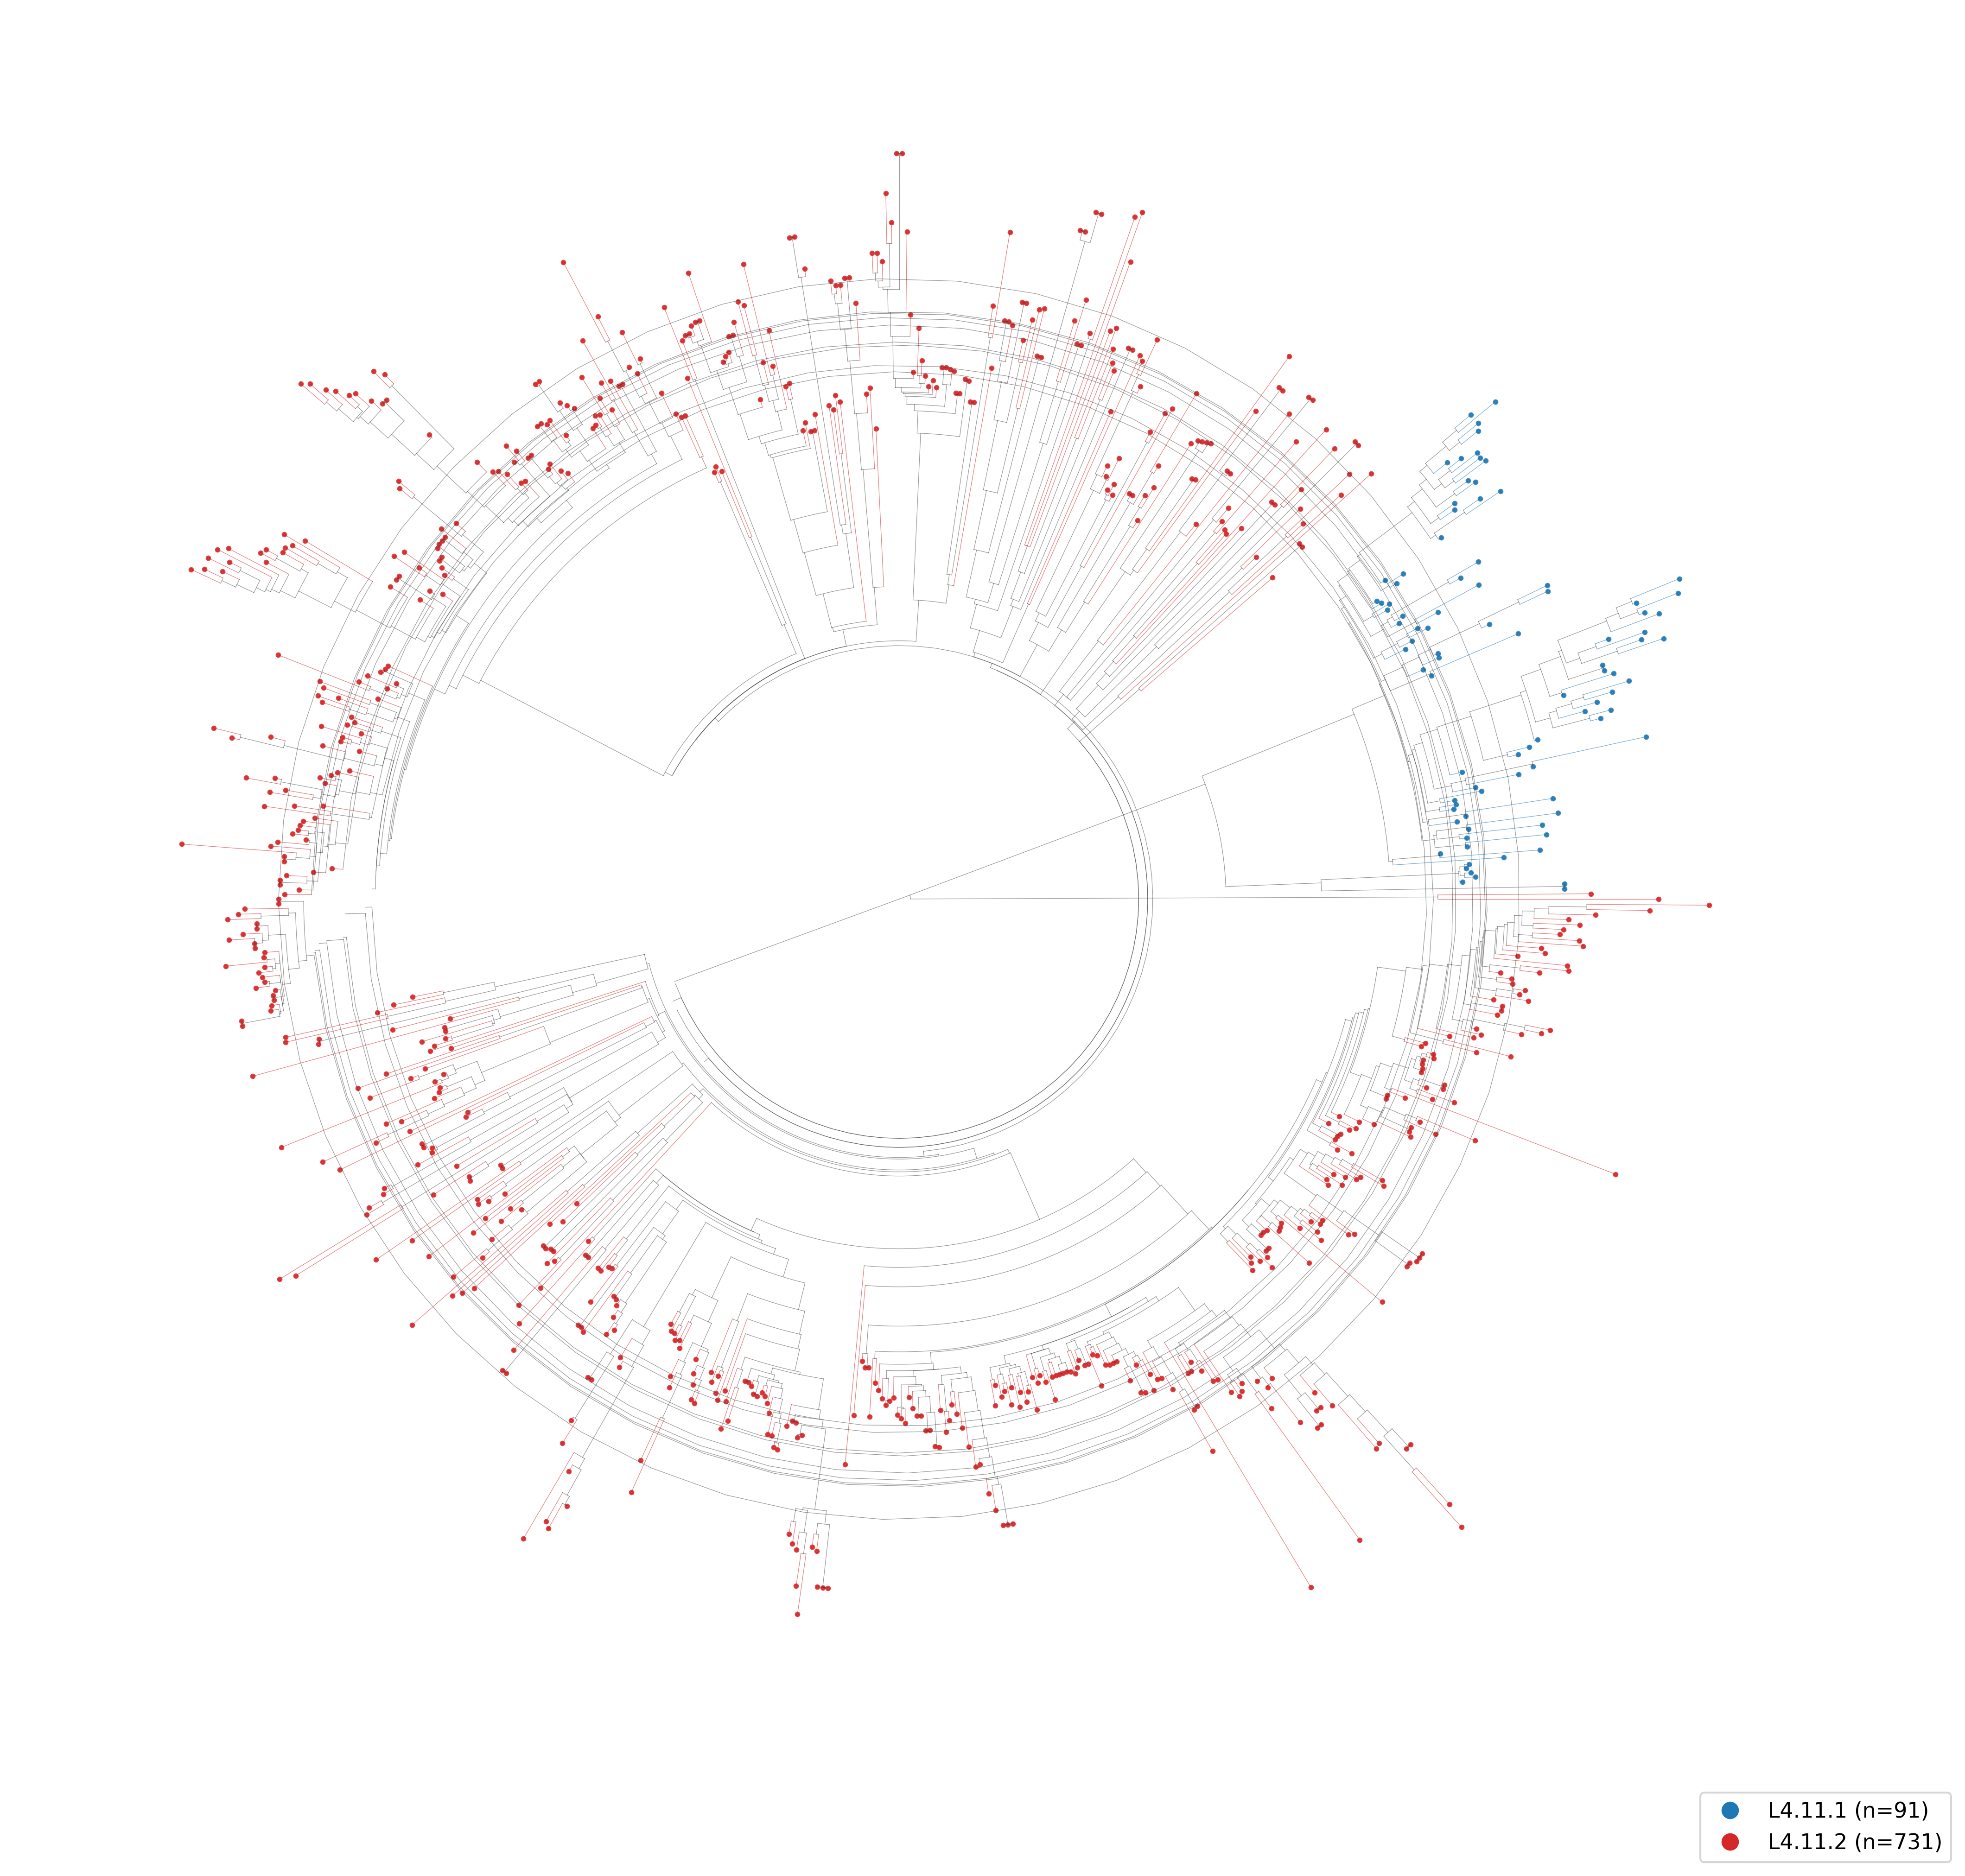
\includegraphics[width=0.85\textwidth]{figures/phylo_tree_l411.png}
	\caption{Midpoint-rooted maximum-likelihood circular phylogeny of the
		825~\lignee{L4.11} SRAs inferred with RAxML-NG (GTR+G4 model).
		Tips are coloured by sub-lineage assignment:
		blue, \lignee{L4.11.1} ($n = 91$);
		red, \lignee{L4.11.2} ($n = 731$).
		Note the deep split between the two sub-lineages and the long
		branch lengths within \lignee{L4.11.1}, consistent with its
		higher marker count (107~core-exclusive SPDIs vs.\ 16).}
	\label{fig:phylo_tree}
\end{figure}
\FloatBarrier

\begin{figure}[htbp!]
	\centering
	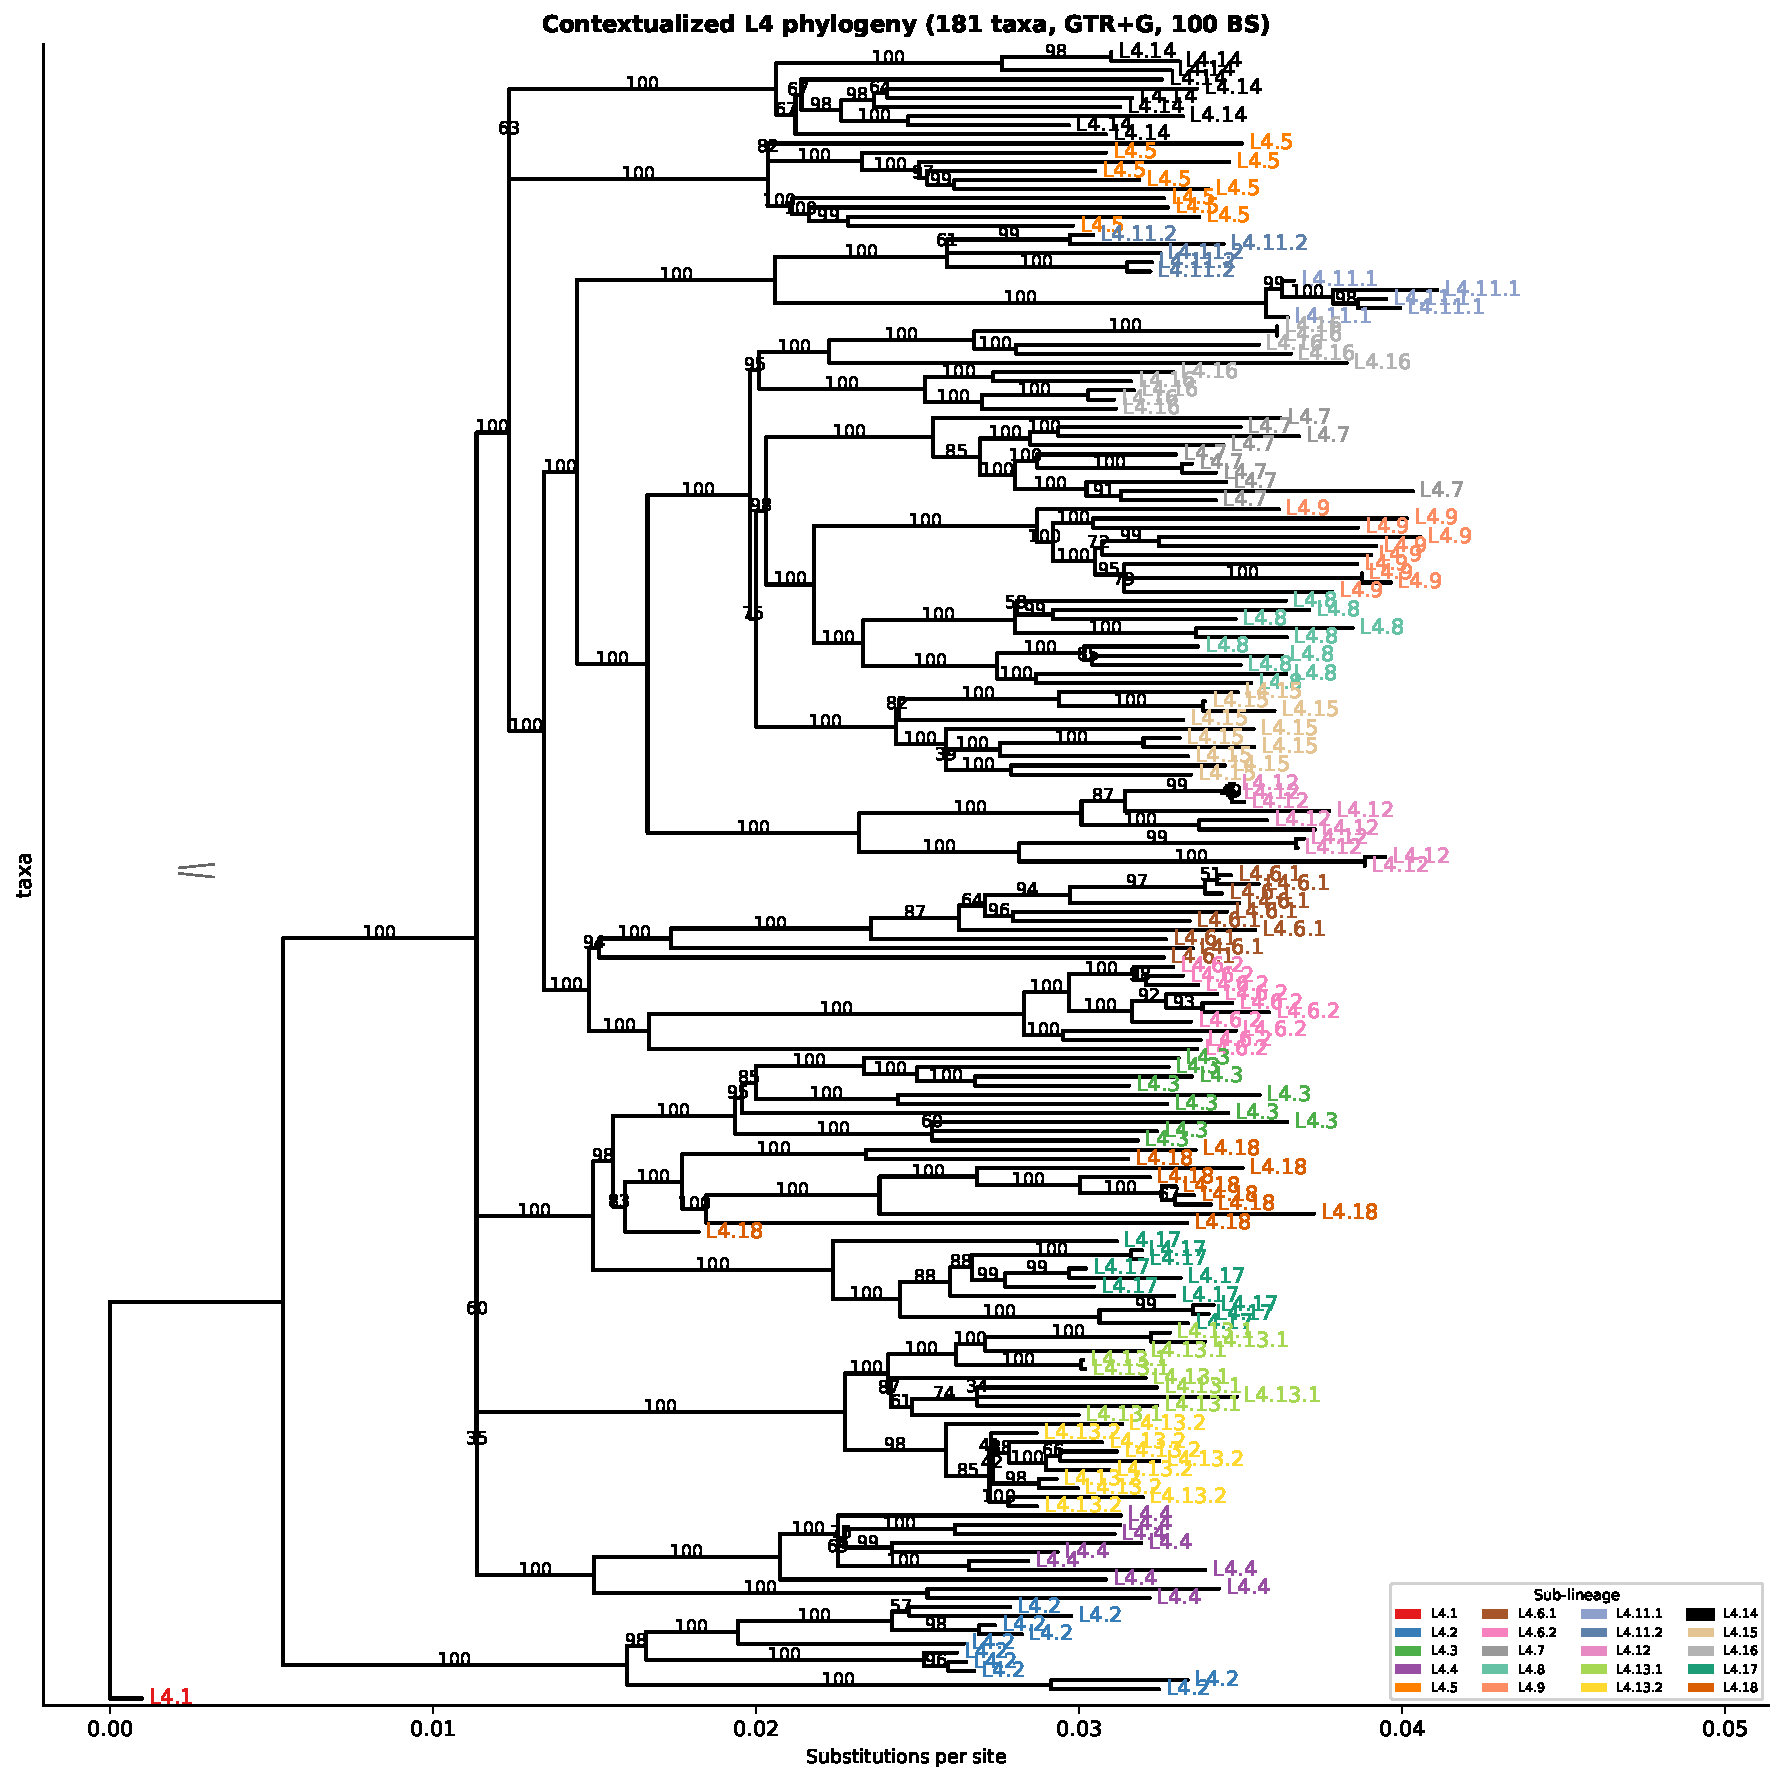
\includegraphics[width=0.92\textwidth]{figures/fig_phylo_L4_context.pdf}
	\caption{Contextualized Lineage~4 phylogeny (181~taxa, GTR+G model, 100~bootstrap replicates). Ten representative SRAs were sampled from each of the 20~L4 sub-lineages (L4.1--L4.18, with L4.11.1 and L4.11.2 treated separately; $n=5$ each). A single L4.1 strain serves as the outgroup. Bootstrap support values are shown at internal nodes.}
	\label{fig:l4_context}
\end{figure}
\FloatBarrier

The maximum-likelihood phylogeny of the 825~\lignee{L4.11} SRAs reveals
a well-resolved tree with two clearly separated sub-clades: \lignee{L4.11.1}
(91~SRAs, 11.0\%) and \lignee{L4.11.2} (731~SRAs, 88.6\%), plus
two deep-branching basal SRAs that lack both
sub-lineage-defining markers.
These basal SRAs --- SRR30679919 (Australia, PRJNA1161723),
SRR33831563 (United States, PRJNA1237251),
occupy a topologically ancestral position.
The two former SRAs share 693~SNPs (171 specific not found in H37Rv) and carry
11~IS6110 copies each, with 10~of 11 insertion positions in common (among which 5 copies are found specifically in these two isolates at positions 36806, 139565, 1987131, 2169199, and 3377387).
They are separated by 150~pairwise SNPs and display two shared small-segment deletions
CUS\_GS\_\allowbreak{}1155829\_\allowbreak{}1155913,
CUS\_GS\_\allowbreak{}3741905\_\allowbreak{}3742046.
Strikingly, the IS6110 insertions in these two basal SRAs predominantly occur in the forward orientation, contrasting with the uniformly reverse orientation of these IS observed in the rest of \lignee{L4.11}
(Section~\ref{sec:structural}).  Their intercontinental spread
(Australia--United States) and deep-branching phylogenetic position
suggest a relict ancestral sister lineage predating the divergence of the two main 4.11 sub-lineages.
The separation between both sub-lineages is confirmed by pairwise
patristic distance analysis (Figure~\ref{fig:heatmap}): inter-group
distances are 4.1$\times$ higher than intra-\lignee{L4.11.1} distances
and 2.2$\times$ higher than intra-\lignee{L4.11.2} distances.
Notably, \lignee{L4.11.1} is markedly more compact (mean patristic
distance 0.0034~subst./site) than \lignee{L4.11.2} (0.0063~subst./site),
consistent with a more recent clonal expansion.

\begin{figure}[htbp!]
	\centering
	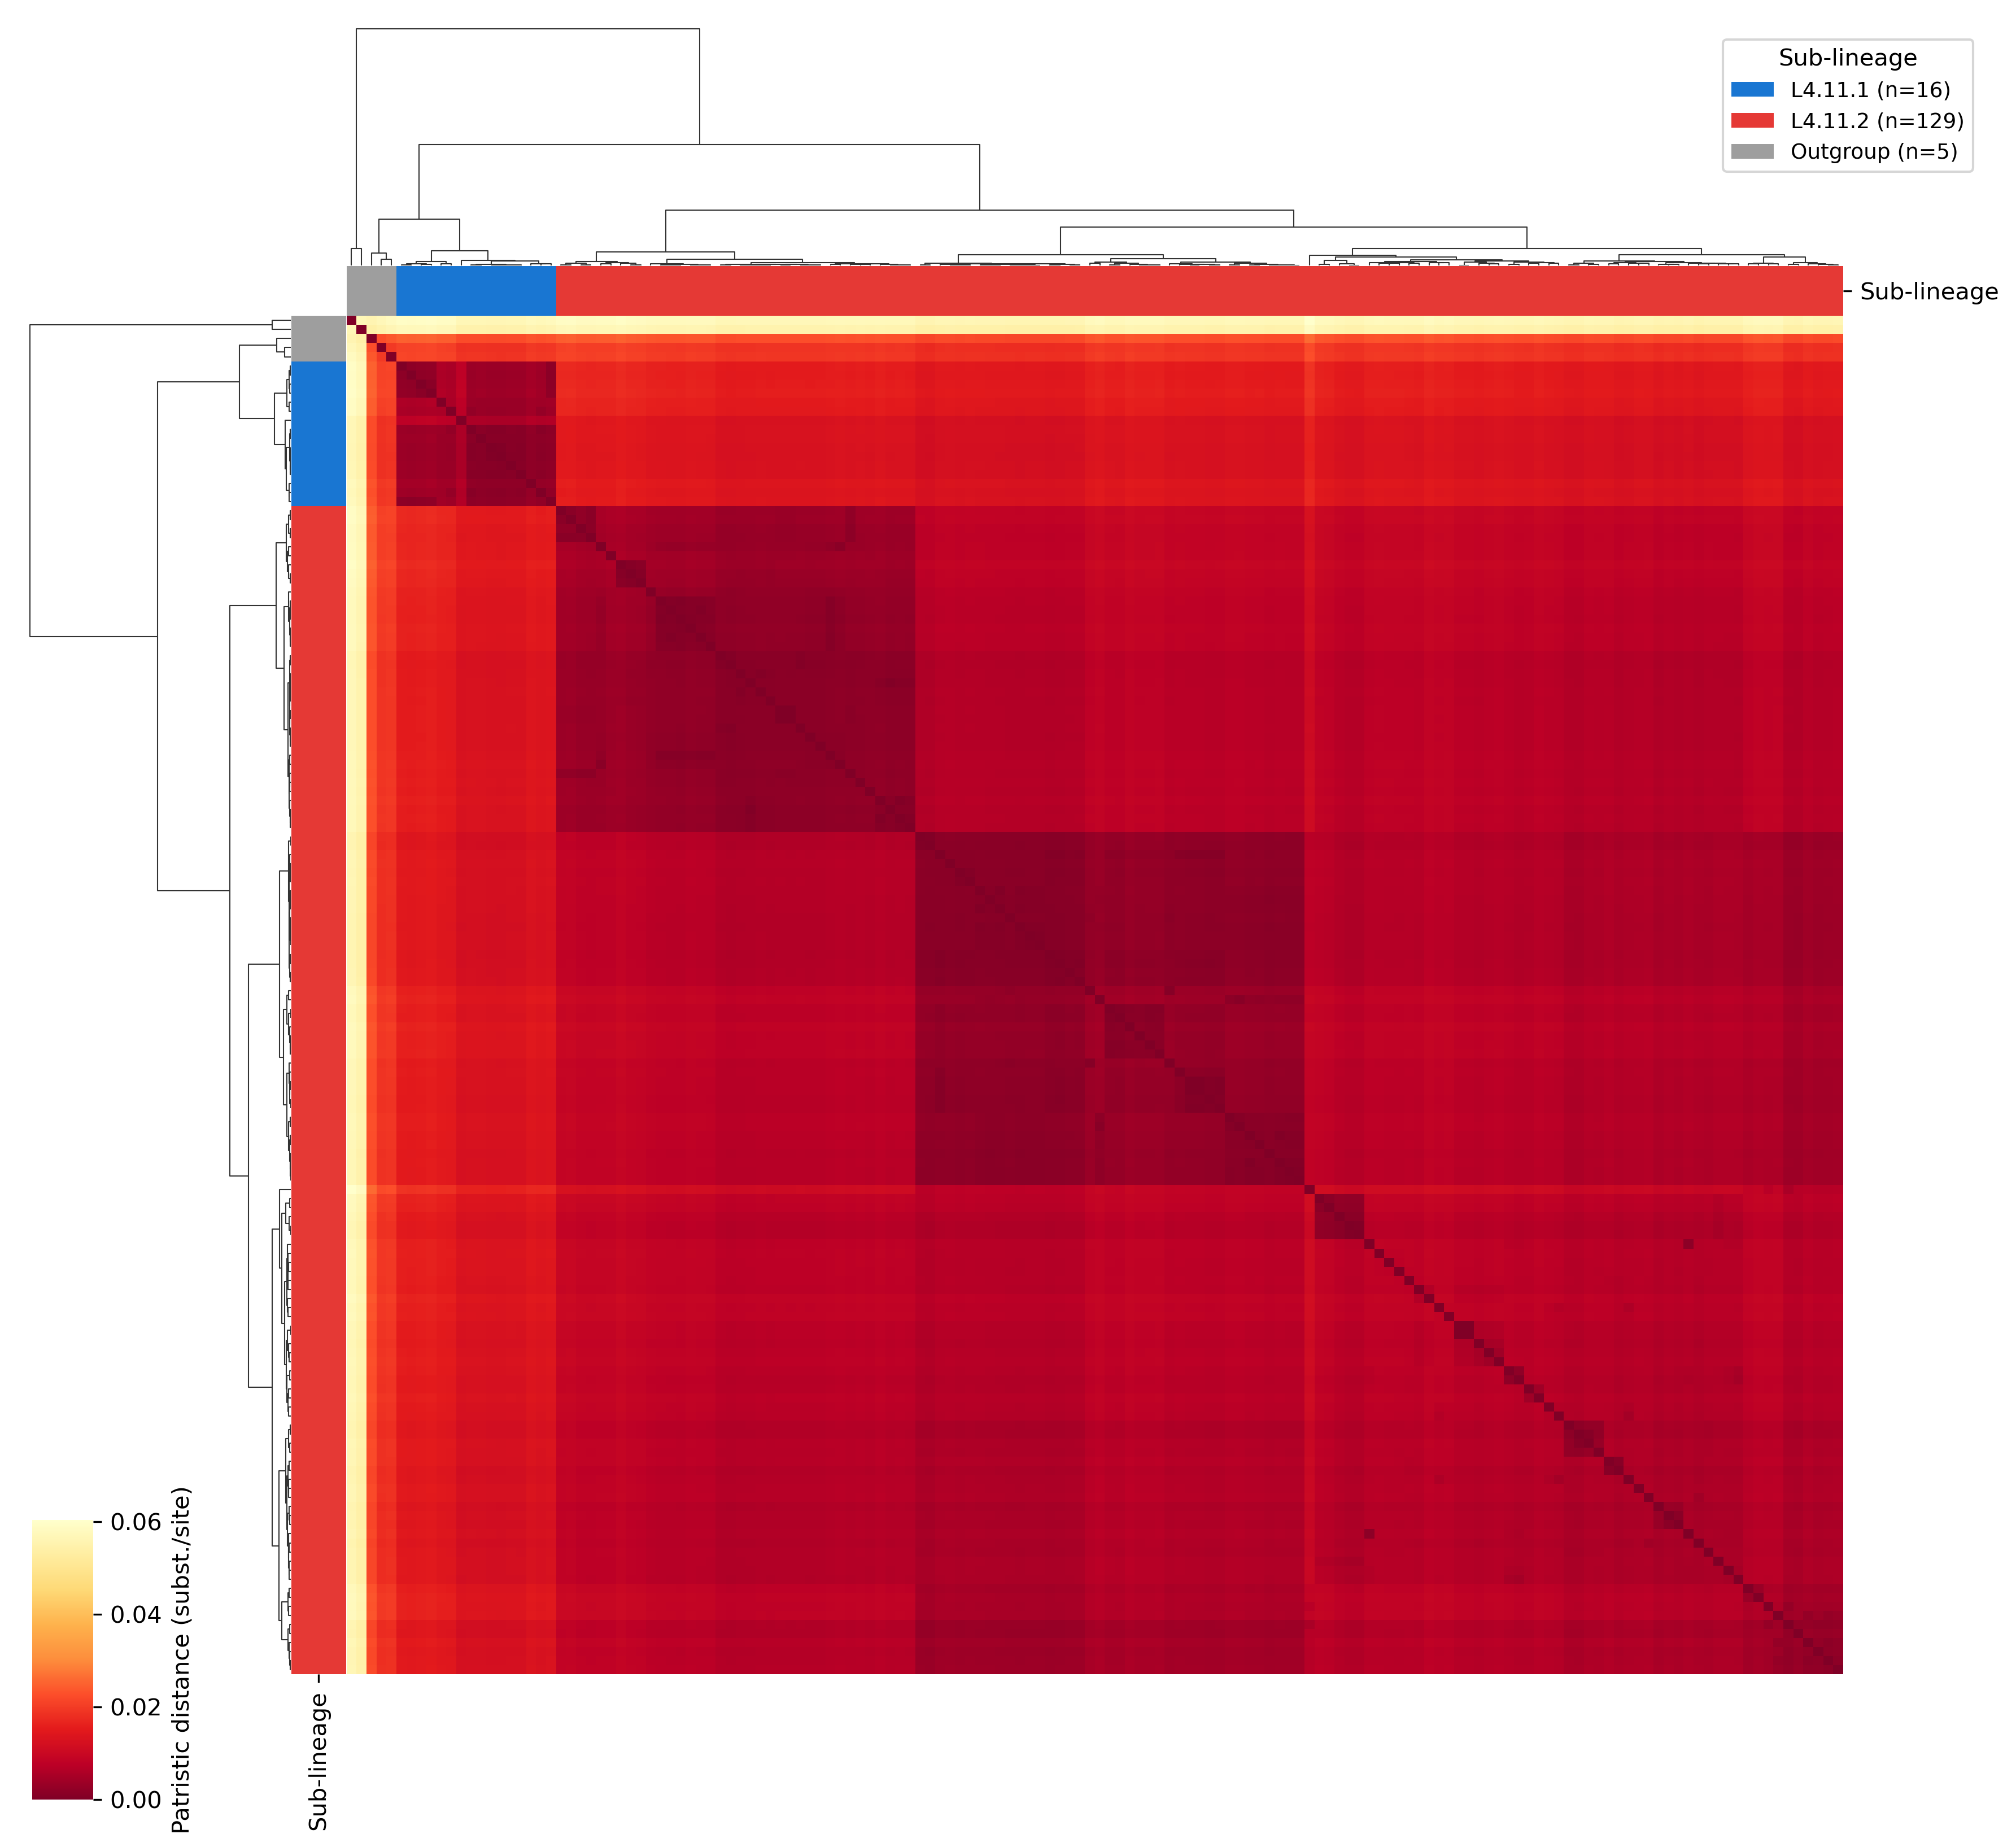
\includegraphics[width=0.63\textwidth]{figures/heatmap_snp_distances.png}
	\caption{Pairwise phylogenetic distance heatmap among \lignee{L4.11} SRAs
		(150~subsampled: 16~\lignee{L4.11.1}, 129~\lignee{L4.11.2}, 5~outgroup).
		Ward hierarchical clustering recovers the two sub-lineages as distinct
		blocks.  Colour bars indicate sub-lineage assignment (blue:
		\lignee{L4.11.1}; red: \lignee{L4.11.2}; grey: outgroup).  Inter-group
		distances (mean $= 0.0138$~subst./site) are 2--4$\times$ higher than
		intra-group distances, confirming the phylogenetic separation.}
	\label{fig:heatmap}
\end{figure}
\FloatBarrier

Principal Coordinates Analysis (PCoA) on the 825~\lignee{L4.11} patristic
distances corroborates the phylogenetic dichotomy
(Figure~\ref{fig:pcoa}).  The first axis (PC1, 43.5\% of variance)
separates \lignee{L4.11.1} from \lignee{L4.11.2}; the second axis
(PC2, 18.2\%) resolves geographic sub-structure within
\lignee{L4.11.2}, where Peruvian, Argentine, and mixed-origin clusters
emerge as distinct clouds.  Bangladeshi isolates form a tight cluster
coinciding with \lignee{L4.11.1}, consistent with the geographic
restriction of this sub-lineage.

\paragraph{A basal ``Proto-\lignee{L4.11.1}'' sub-clade.}

Within the \lignee{L4.11.1} clade, a basal sub-clade of 7~isolates
(5~from South Africa, 2~from the United Kingdom) is sister to the
84-strain core that dominates Bangladesh
(Figure~\ref{fig:pcoa}a, green triangles).  One South African isolate
(SRR35281599) carries the spoligotype SIT358 (octal 717777777760771,
SITVIT2 clade T1), a pattern historically associated with Bangladesh
and East Africa, and described in 1995 for the first time (http://www.pasteur-guadeloupe.fr:8081/SITVIT2/query).  The five South African SRAs originate from a
household transmission study (BioProject PRJNA1312808, ``HoTT DCTB'').
All 7~Proto-\lignee{L4.11.1} SRAs carry a novel IS6110 insertion
at position 2\,627\,395 in the forward orientation, a unique
synapomorphic marker for this sub-clade.  This position lies within an
IS6110 insertion hotspot: 43~\lignee{L4.11.2} SRAs carry a nearby
reverse-oriented copy at position 2\,626\,859, and a broader database
search identifies 27~SRAs with forward and 15~with reverse IS6110
copies within this locus.  The co-occurrence of both orientations at a
single hotspot is one of the few exceptions to the otherwise uniform
reverse-only IS6110 insertion pattern across \lignee{L4.11}
(Section~\ref{sec:structural}).
This basal positioning and geographic spread, as well as more ancient results obtained using spoligotyping results suggest that the ancestor
of \lignee{L4.11.1} had a wider distribution before the clonal
expansion became centered on Bangladesh (e.g in Ethiopia, Sudan, Turkey).

\begin{figure}[htbp!]
	\centering
	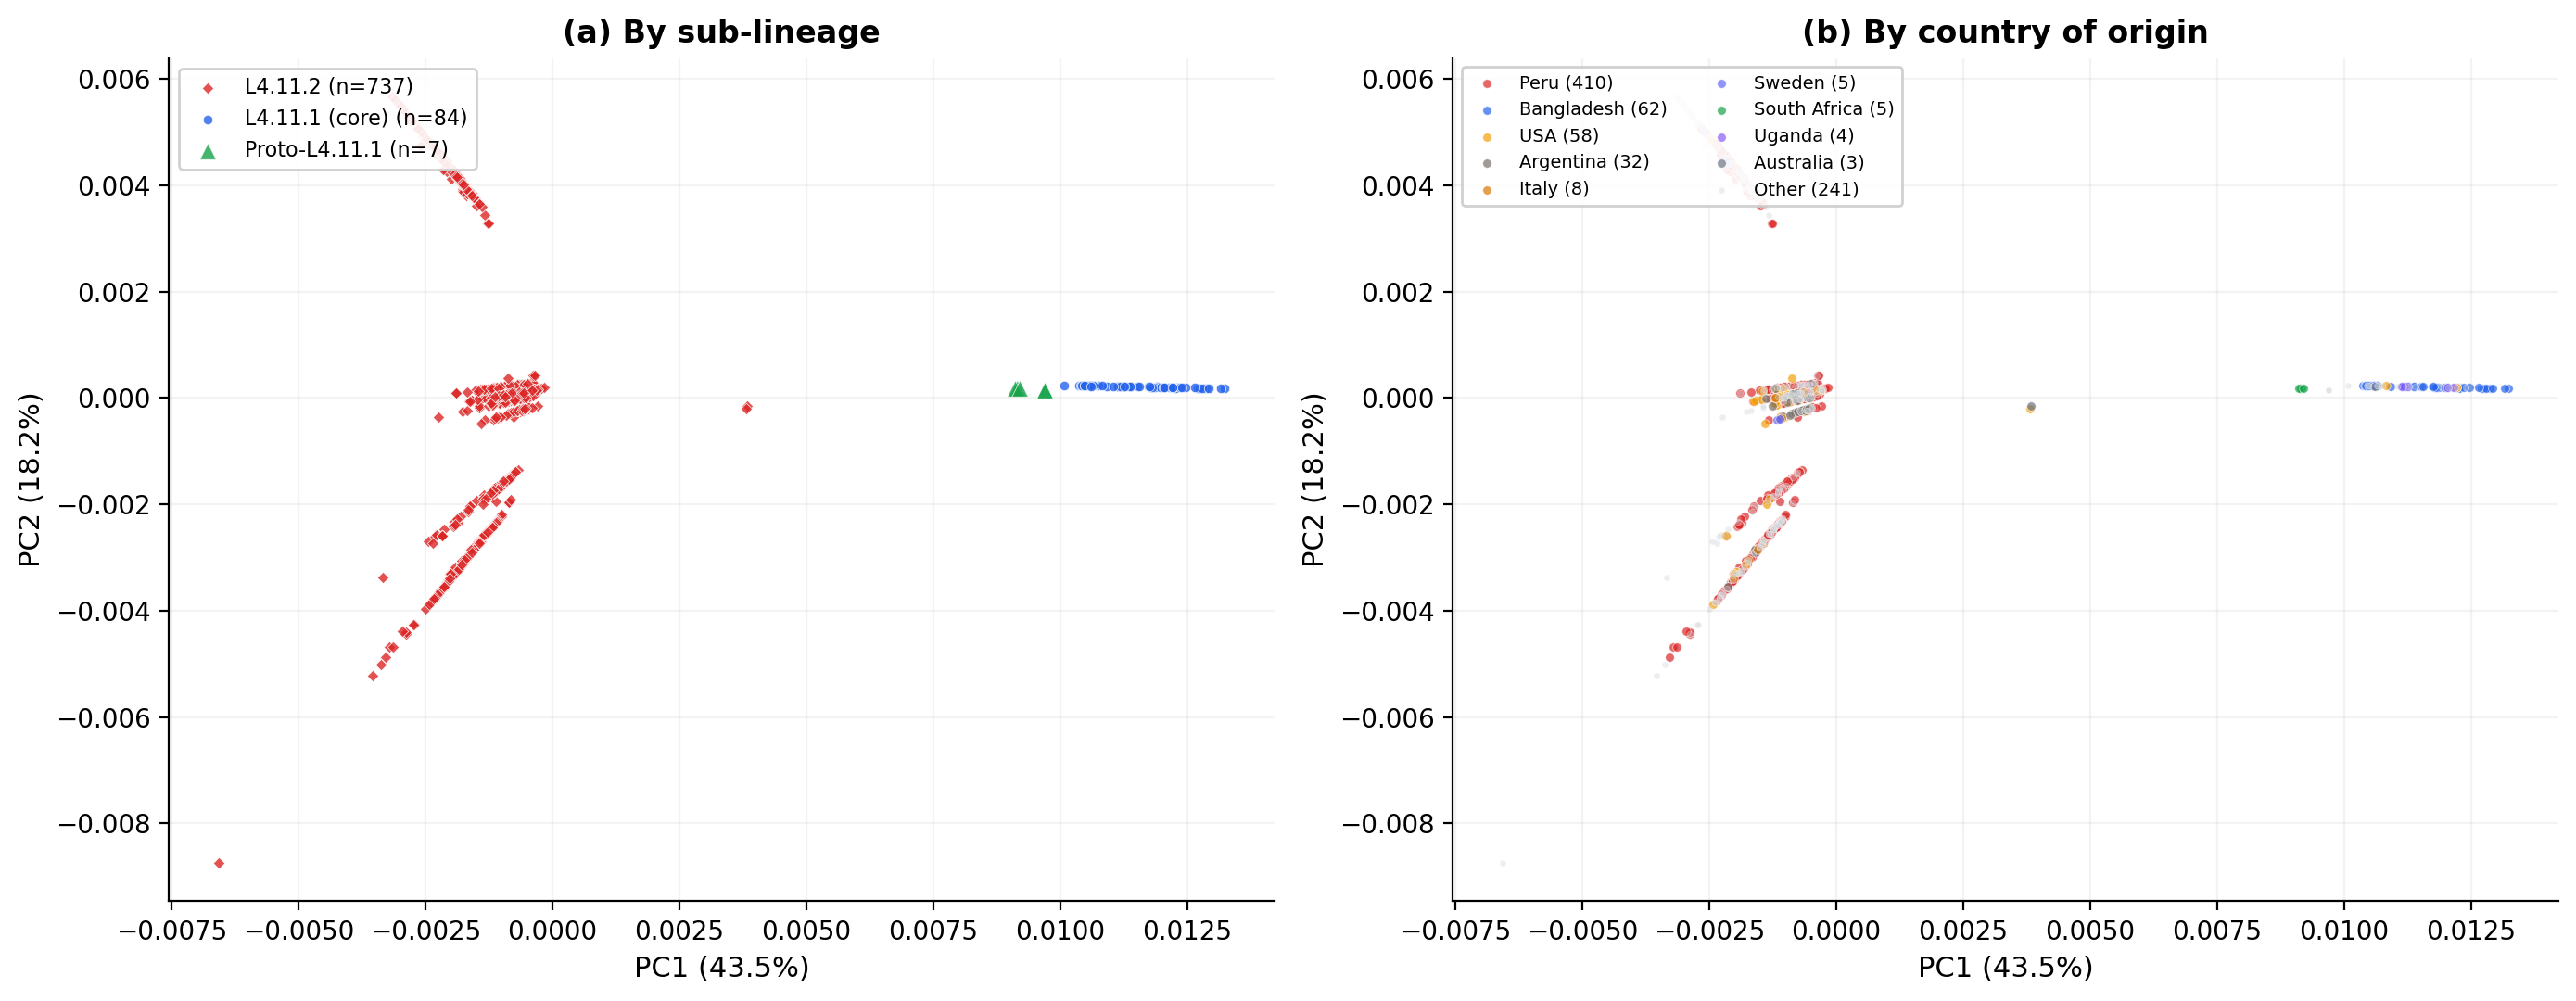
\includegraphics[width=0.85\textwidth]{figures/pcoa_l411.png}
	\caption{Principal Coordinates Analysis of 825~\lignee{L4.11} SRAs
		based on patristic distances.
		\textbf{(a)}~Coloured by sub-group: blue circles,
		core \lignee{L4.11.1} ($n = 84$); green triangles,
		Proto-\lignee{L4.11.1} ($n = 7$; 5~South Africa, 2~UK);
		red diamonds, \lignee{L4.11.2} and basal SRAs ($n = 734$).
		\textbf{(b)}~Coloured by country of origin (top~9 countries shown).
		PC1 (43.5\%) separates the two sub-lineages; PC2 (18.2\%)
		resolves geographic sub-clusters within \lignee{L4.11.2}.}
	\label{fig:pcoa}
\end{figure}
\FloatBarrier

\paragraph{Core-exclusive markers.}

A total of 214~core SPDIs were identified (present in all 825~SRAs).
Among these, 8~core-exclusive SPDIs are absent from all SRAs outside
\lignee{L4.11}, providing unambiguous molecular markers for this sub-lineage
(Table~\ref{tab:core_excl}).  We propose the combination of
\spdi{NC\_000962.3:1374351:C:T} (Rv1231c, E171D) and
\spdi{NC\_000962.3:1800962:C:T} (\textit{hisC1}, A23V)
as the defining barcode for \lignee{L4.11}.

\begin{table}[ht]
	\centering
	\caption{Core-exclusive SPDIs defining \lignee{L4.11} (8~markers, all on
		chromosome \spdi{NC\_000962.3}).}
	\label{tab:core_excl}
	\begin{tabular}{rllll}
		\toprule
		\textbf{Pos.} & \textbf{SPDI}      & \textbf{Gene}       & \textbf{Effect} & \textbf{Product}                      \\
		\midrule
		13\,074        & \spdi{13073:G:A}   & \textit{ppiA}/Rv0010c & intergenic     & Peptidyl-prolyl isomerase region       \\
		787\,680      & \spdi{787679:C:T}  & Rv0687              & syn             & NAD-dependent oxidoreductase          \\
		1\,116\,007   & \spdi{1116006:A:G} & Rv0999              & T81A            & Hypothetical protein                  \\
		1\,374\,352   & \spdi{1374351:C:T} & Rv1231c             & E171D           & Membrane protein                      \\
		1\,800\,963   & \spdi{1800962:C:T} & \textit{hisC1}      & A23V            & Histidinol-phosphate aminotransferase \\
		3\,505\,751   & \spdi{3505750:C:T} & \textit{fadE24}     & P130L           & Acyl-CoA dehydrogenase                \\
		3\,957\,395   & \spdi{3957394:A:G} & Rv3529c             & intragenic      & Hypothetical protein                  \\
		4\,328\,317   & \spdi{4328316:G:A} & \textit{ethR}/3856c & intergenic      & ethR regulatory region                \\
		\bottomrule
	\end{tabular}
\end{table}

Three additional markers that were core-exclusive in the initial v2 dataset
(415~SRAs) lost this status upon dataset enrichment: \spdi{1483362:C:T}
(Rv1320c, adenylate cyclase), \spdi{1899138:C:T} (Rv1673c), and
\spdi{2778941:G:A} (Rv2476c/\textit{gdh}).  This underscores the importance of
validating barcode markers exclusivity across large, independently assembled datasets.

\paragraph{Concordance with existing nomenclatures.}

We cross-referenced the 8~exclusive SNPs of \lignee{L4.11}
(Table~\ref{tab:core_excl}) with five established classification
systems.  All systems assign \lignee{L4.11} SRAs to broadly
concordant positions within L4: Coll~4/4.9,
Napier~4/4.9, Shitikov~4/4.9, and Stucki~4.10.  In the Freschi system,
731~SRAs (all \lignee{L4.11.2}) are assigned to Freschi~4.11, while
the remaining 94~SRAs (\lignee{L4.11.1} and basal) fall at the
unresolved level~4; notably, \lignee{L4.11} is \emph{not} within
Freschi~4.10.i2, which corresponds to a separate clade centred on
H37Rv and the naming of L4.11 was wrongly attributed to a peruvian epidemic sub-clade.  None of the current classification systems resolved the full \lignee{L4.11} clade as
a distinct entity, confirming that if, it represented a previously detected
sub-lineage, its description was only relative to an limited epidemic clone. The mmpL5 frameshift variant found at position 777875:AC:A is indeed found exclusively in a subbranch of L4.11.2 that represents the most recently emerged sublone of L4.11.2, and whose maximum distance between two isolates is never superior to 90 SNPs (mean : 34 +/-12 SNPs) \cite{vargas2021,freschi2021}.

\paragraph{Sub-lineage L4.11.1.}

Within \lignee{L4.11}, a robust sub-lineage emerges from the
phylogenetic analysis: L4.11.1.  \lignee{L4.11.1} \textit{sensu lato}, (i.e. including the 7 proto L4.11.1) comprises 91~SRAs (11.0\% of
\lignee{L4.11}) and is supported by 530~shared SNPs (present in all
91~SRAs), of which 107~are exclusive to \lignee{L4.11.1}
within the \lignee{L4.11} dataset and absent from all
\lignee{L4.11.2} SRAs (Table~\ref{tab:l4111}).
When exclusivity is evaluated against the broader L4 lineage,
69~of these markers remain absent from all non-\lignee{L4.11.1}
SRAs, confirming the robustness of this sub-lineage definition.

\begin{table}[ht]
	\centering
	\caption{Summary of \lignee{L4.11.1}.}
	\label{tab:l4111}
	\begin{tabular}{lr}
		\toprule
		\textbf{Property}    & \textbf{Value}               \\
		\midrule
		Number of SRAs    & 91                           \\
		Proportion of L4.11  & 11.0\%                       \\
		Shared SNPs           & 530                          \\
		Exclusive SNPs        & 107 (69 vs.\ all L4)         \\
		Defining barcode     & \spdi{33084:C:T} + \spdi{1700209:G:A}  \\
		Including indels     & 3 (GT ins., C del., CA ins.) \\
		\bottomrule
	\end{tabular}
\end{table}

\lignee{L4.11.1} is not captured by any existing classification system below
the level of Coll~4.9 / Stucki~4.10 (of which
\lignee{L4.11} is a sub-group), confirming it as a
novel sub-lineage.  We propose the combination of
\spdi{NC\_000962.3:33084:C:T} (Rv0031, Q199Q) and
\spdi{NC\_000962.3:1700209:G:A} (Rv1508A)
as a potential defining barcode for \lignee{L4.11.1}.

The core-exclusive set also includes three more insertion/deletion variants:
\spdi{1713356:G:GT}, \spdi{1993200:AA:C}, and \spdi{2379599:C:CA},
further characerizing this sublineage.

\paragraph{Sub-lineage L4.11.2.}

The complement of \lignee{L4.11.1} within \lignee{L4.11} forms a second
well-supported sub-lineage.  \lignee{L4.11.2} comprises 731~SRAs
(88.6\% of \lignee{L4.11}) and is defined by 16~core-exclusive markers
(Table~\ref{tab:l4112}).

\begin{table}[ht]
	\centering
	\caption{Core-exclusive SPDIs defining \lignee{L4.11.2} (16~markers).}
	\label{tab:l4112}
	\footnotesize
	\begin{tabular}{rllll}
		\toprule
		\textbf{Pos.} & \textbf{SPDI}      & \textbf{Gene}        & \textbf{Effect} & \textbf{Product}                \\
		\midrule
		130\,083      & \spdi{130082:A:C}  & \textit{ctpI}        & syn             & Cation-transporter ATPase I     \\
		613\,989      & \spdi{613988:T:C}  & \textit{gabP}        & S318P           & GABA permease                   \\
		761\,889      & \spdi{761888:G:C}  & \textit{rpoB}        & V695L           & RNA polymerase $\beta$ subunit  \\
		812\,339      & \spdi{812338:T:C}  & \textit{rplE}        & V94A            & 50S ribosomal protein L5        \\
		1\,285\,148   & \spdi{1285147:G:A} & \textit{pimE}        & G53S            & PIM mannosyltransferase         \\
		2\,223\,214   & \spdi{2223213:T:G} & \textit{mpt64}/1979c & intergenic      & Immunogenic secreted protein    \\
		2\,333\,753   & \spdi{2333752:T:G} & Rv2077c              & Q181P           & Transmembrane protein           \\
		2\,827\,364   & \spdi{2827363:G:A} & \textit{orn}         & D70N            & Oligoribonuclease               \\
		2\,982\,158   & \spdi{2982157:C:T} & Rv2664               & A21V            & Hypothetical protein            \\
		3\,065\,517   & \spdi{3065516:G:A} & Rv2752c              & syn             & Conserved hypothetical          \\
		3\,340\,871   & \spdi{3340870:G:T} & \textit{ppk1}        & G340C           & Polyphosphate kinase            \\
		3\,505\,708   & \spdi{3505707:A:C} & \textit{fadE24}      & I116L           & Acyl-CoA dehydrogenase          \\
		3\,630\,854   & \spdi{3630853:A:T} & \textit{alkB}        & W379R           & Alkane 1-monooxygenase          \\
		4\,216\,745   & \spdi{4216744:T:C} & \textit{hisC2}/3771c & intergenic      & Near histidine aminotransferase \\
		4\,286\,551   & \spdi{4286550:G:A} & Rv3821               & syn             & Integral membrane protein       \\
		4\,397\,020   & \spdi{4397019:C:T} & Rv3910               & syn             & Transmembrane protein           \\
		\bottomrule
	\end{tabular}
\end{table}

\lignee{L4.11.2} has 160~core SPDIs overall.  Like \lignee{L4.11.1}, it is
not captured by any existing classification system below the level of
Coll~4.9.  We propose the combination of \spdi{NC\_000962.3:143666:C:T}
(\textit{oxcA}, Rv0118c) and \spdi{NC\_000962.3:801008:A:G}
(Rv0693, A29A) as the defining barcode for
\lignee{L4.11.2}.  This sublineage is a larger sublineage than the one designated
as Freschi~4.11, which was studied by Vargas~\textit{et al.} in the
context of epistasia of drug-resistance mutations ~\cite{vargas2021}.

The functional annotation of the 16~core-exclusive markers reveals a
striking profile enriched in drug-target and lipid metabolism genes.
The \textit{rpoB} V695L mutation affects the rifampicin target (outside
the canonical RRDR), while \textit{fadE24} I116L alters an acyl-CoA
dehydrogenase involved in lipid degradation and flagged for isoniazid
resistance by Mycobrowser.  The \textit{alkB} W379R mutation
(tryptophan$\to$arginine) disrupts fatty acid $\omega$-hydroxylation,
and \textit{pimE} G53S affects phosphatidylinositol mannoside (PIM)
biosynthesis --- a key component of the mycobacterial cell envelope.
The \textit{rplE} V94A mutation targets the 50S ribosomal protein~L5,
and \textit{gabP} S318P alters a GABA permease involved in
$\gamma$-aminobutyrate transport.  Together with the \textit{ppk1}
G340C (persistence/biofilm), \textit{orn} D70N (stringent response),
and the dual \textit{hisC} perturbation, these markers define
a lineage with concurrent alterations in lipid metabolism, translation,
cell envelope biogenesis, and stress response.

\subsection{Geographic distribution}

Geographic metadata was available for 591 of 825~SRAs (71.6\%), spanning
14~countries on 5~continents.  The two sub-lineages exhibit a striking
phylogeographic partition (Table~\ref{tab:geo}).

\begin{table}[ht]
	\centering
	\caption{Geographic distribution of \lignee{L4.11} sub-lineages
		(SRAs with available metadata).}
	\label{tab:geo}
	\begin{tabular}{lrrr}
		\toprule
		\textbf{Country}       & \textbf{L4.11.1} & \textbf{L4.11.2} & \textbf{Total} \\
		\midrule
		Peru                   & ---              & 410              & 410            \\
		Bangladesh             & 62               & ---              & 62             \\
		USA                    & 3                & 55               & 58             \\
		Argentina              & ---              & 32               & 32             \\
		Italy                  & ---              & 8                & 8              \\
		South Africa           & 5                & ---              & 5              \\
		Sweden                 & ---              & 5                & 5              \\
		Uganda                 & 4                & ---              & 4              \\
		Australia              & 1                & 2                & 3              \\
		United Kingdom         & 2                & ---              & 2              \\
		Other (2~countries)    & ---              & 2                & 2              \\
		\midrule
		\textbf{Total (known)} & \textbf{77}      & \textbf{514}     & \textbf{591}   \\
		Unknown                & 14               & 220              & 234            \\
		\bottomrule
	\end{tabular}
\end{table}

\lignee{L4.11.2} is strongly associated with South America, particularly
Peru (80.1\% of SRAs with metadata), consistent with the Lima-based MDR
cluster described by Vargas \textit{et al.}.and Freschi \textit{et al.} ~\cite{vargas2021,freschi2021}.  In contrast,
\lignee{L4.11.1} is predominantly found in Bangladesh (80.5\%) and
East Africa (South Africa, Uganda), suggesting a distinct epidemiological
niche centred on South Asia.

This phylogeographic partition is statistically highly significant.
A $\chi^2$ test on the 10-country contingency table
(Table~\ref{tab:geo}) yields $\chi^2 = 648.5$, $\mathrm{df} = 9$,
$p < 10^{-133}$ (Cram\'er's~$V = 0.89$), indicating a near-perfect
association between country and sub-lineage.
Per-country Fisher exact tests (Bonferroni-corrected)
confirm that Bangladesh is exclusively associated with \lignee{L4.11.1}
($p_{\mathrm{Bonf}} < 10^{-70}$), Peru with \lignee{L4.11.2}
($p_{\mathrm{Bonf}} < 10^{-29}$), and both South Africa
($p_{\mathrm{Bonf}} = 1.5 \times 10^{-4}$)
and Uganda ($p_{\mathrm{Bonf}} = 1.4 \times 10^{-3}$) with
\lignee{L4.11.1}.

\begin{figure}[htbp!]
	\centering
	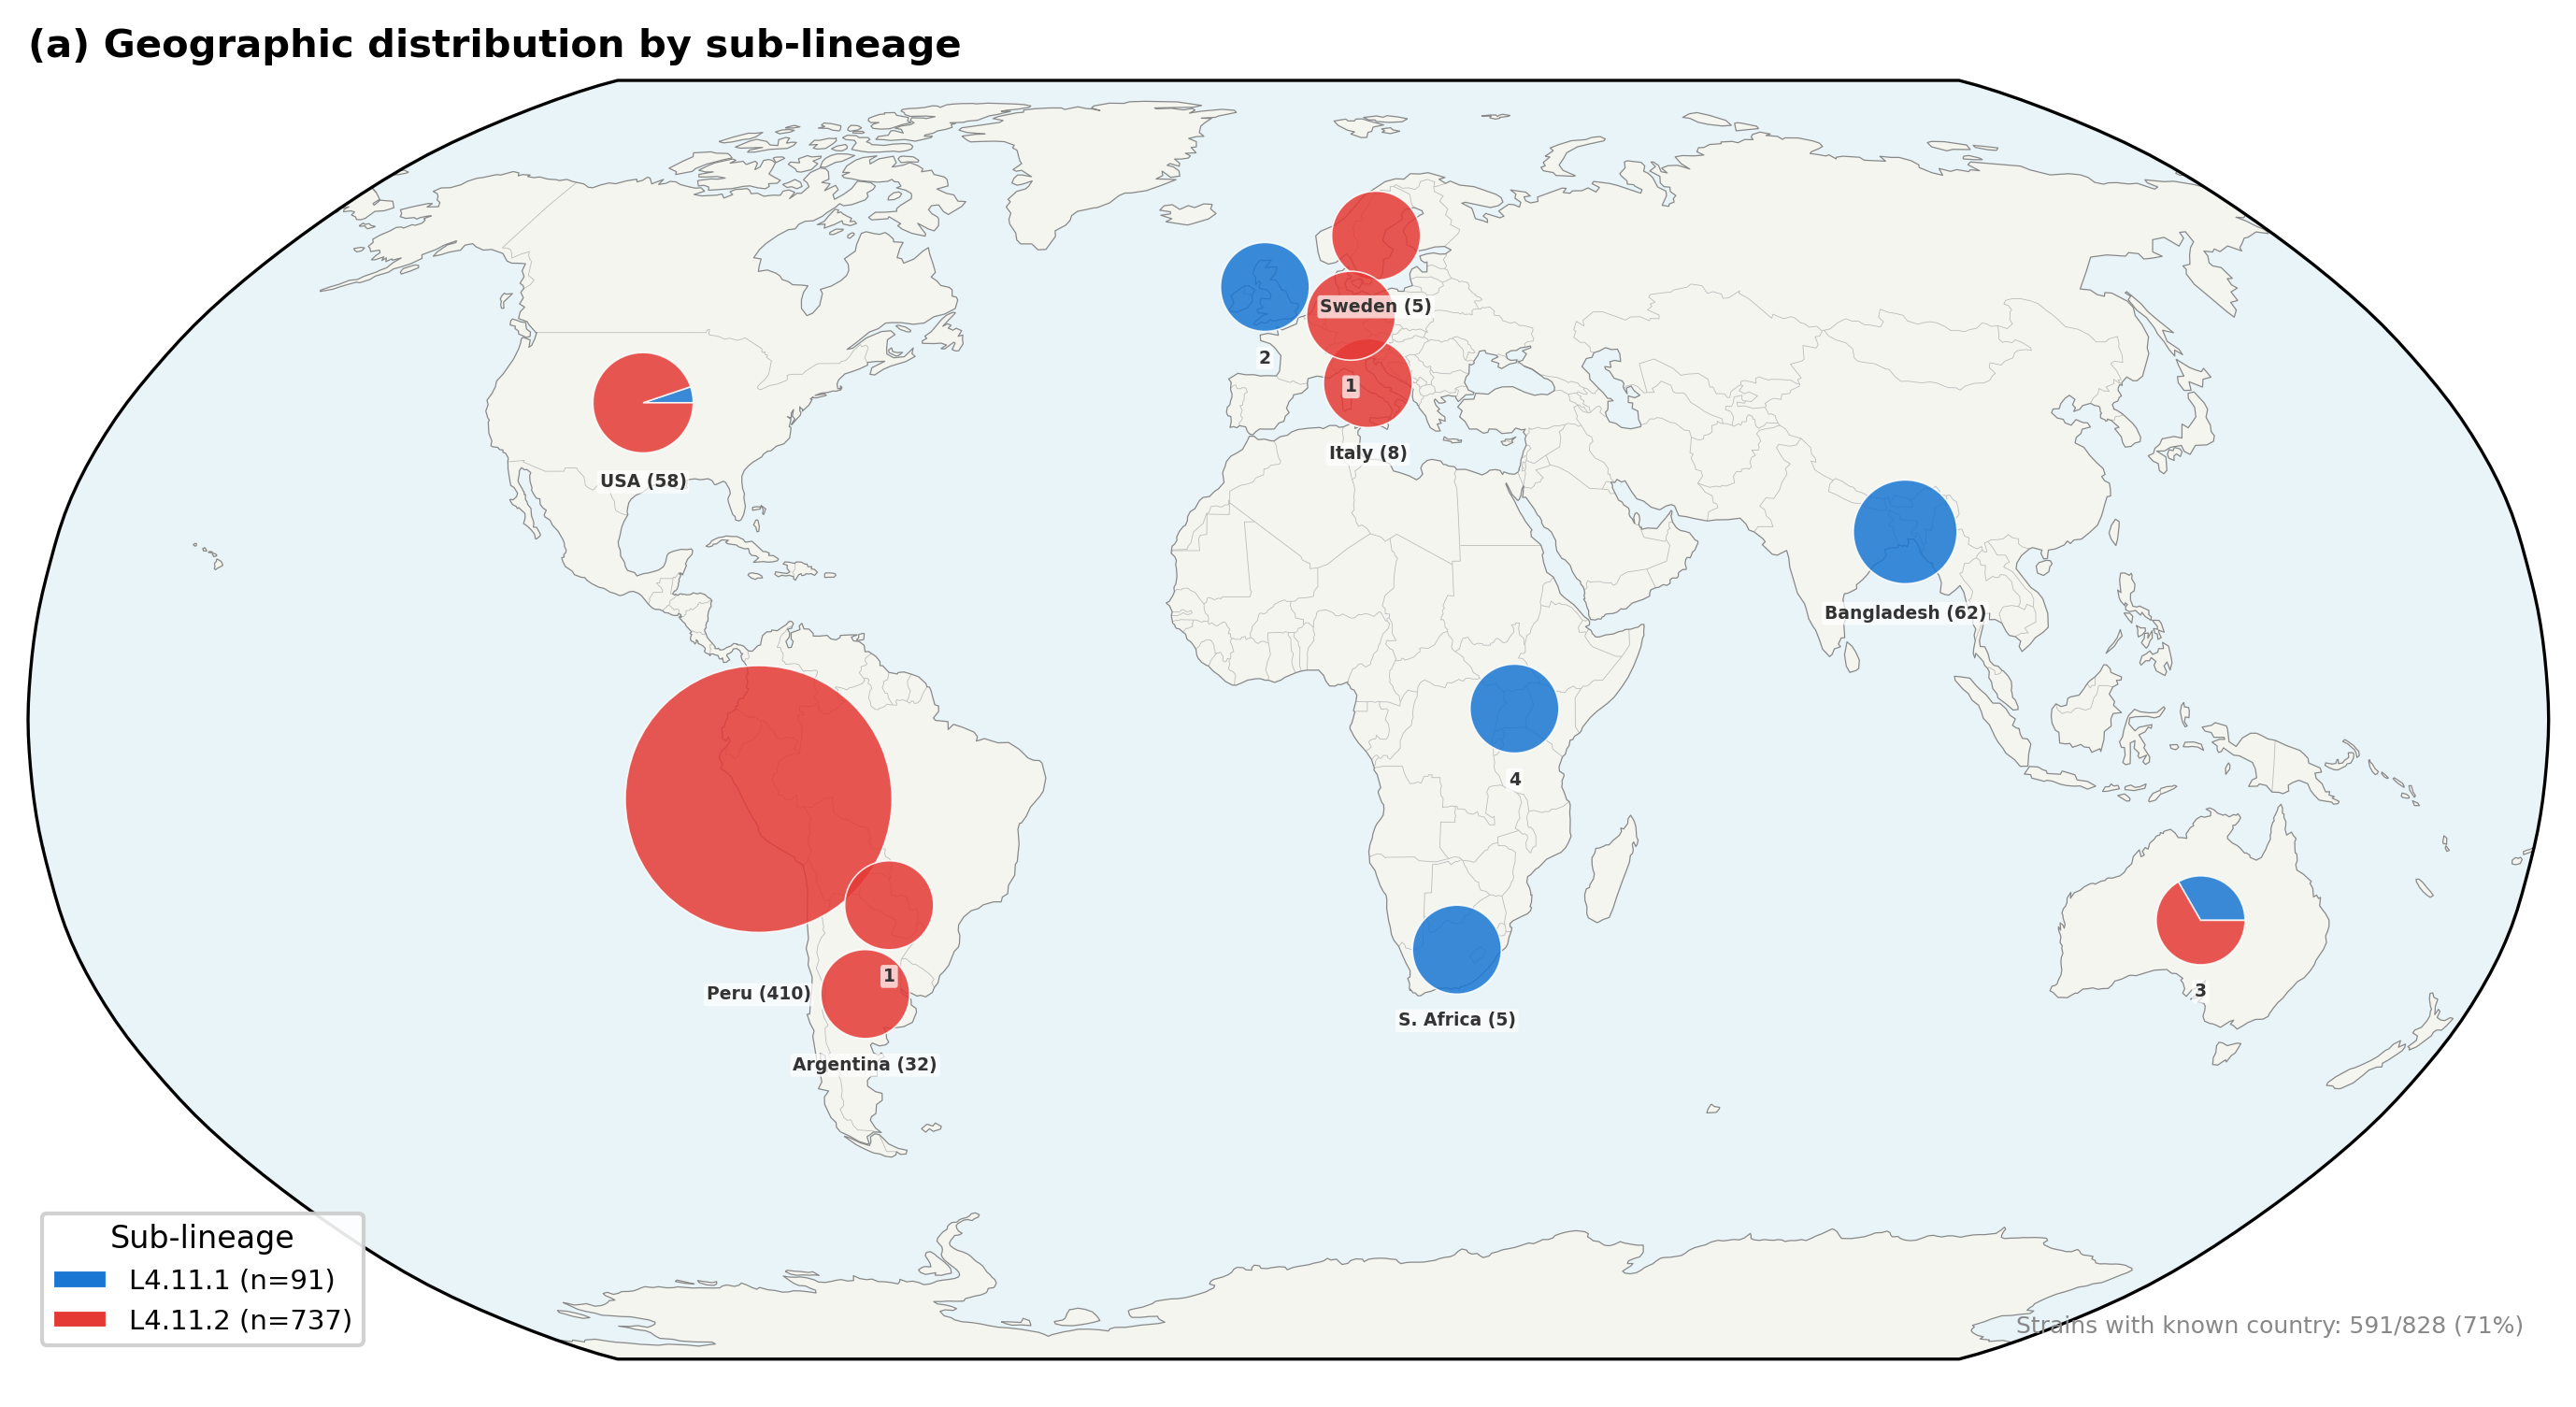
\includegraphics[width=0.65\textwidth]{figures/map_l411_geographic.png}
	\caption{Geographic distribution of \lignee{L4.11} sub-lineages.
		Pie charts show the relative proportions of \lignee{L4.11.1} (blue)
		and \lignee{L4.11.2} (red); chart area is proportional to strain
		count (591~SRAs with known country out of 825).}
	\label{fig:geographic}
\end{figure}
\FloatBarrier

\subsection{Spoligotype analysis}

\textit{In silico} spoligotyping of all 825~SRAs reveals distinctive
CRISPR spacer deletion patterns that mirror the SNP-based sub-lineage
structure (Figure~\ref{fig:spoligo}).
The canonical spacer~33-36 are absent in 100\% of \lignee{L4.11} SRAs,
a hallmark of the T1 spoligotype family, while spacers~34--36 are
virtually absent in \lignee{L4.11.1} ($<$\,5\%) but retained in
\lignee{L4.11.2} ($\le$\,1\%).
Spacers~4 and~5 provide additional sub-lineage discrimination:
spacer~5 is uniformly absent in \lignee{L4.11.1} and
Proto-\lignee{L4.11.1} (0\%) but present in 68.4\% of
\lignee{L4.11.2} SRAs, indicating an early deletion event in the
L4.11.1 ancestor.

The most frequent spoligotype pattern in \lignee{L4.11.2}
(121~SRAs, 16.5\%) retains all spacers except 33--36, corresponding
to the classical T1 family.  Spoligotype diversity is high across both
sub-lineages: 382~unique patterns were observed among 825~SRAs, and
only 3~SRAs could be assigned to a known SIT\@.
This high orphan rate is typical of \textit{in silico} spoligotyping
from WGS data, where micro-variations in CRISPR loci generate
patterns not present in the SITVIT2 database~\cite{couvin2019}.
Quantitative analysis of CRISPR spacer coverage further revealed that
several DR spacers (DR2, DR4--DR7) exhibit partial coverage
(0.05--0.3$\times$ genome depth) in 40--76\% of \lignee{L4.11.2} SRAs
but are uniformly absent in \lignee{L4.11.1}, suggesting ongoing mosaic
erosion of the CRISPR locus specific to the Peruvian sub-lineage.

\begin{figure}[htbp!]
	\centering
	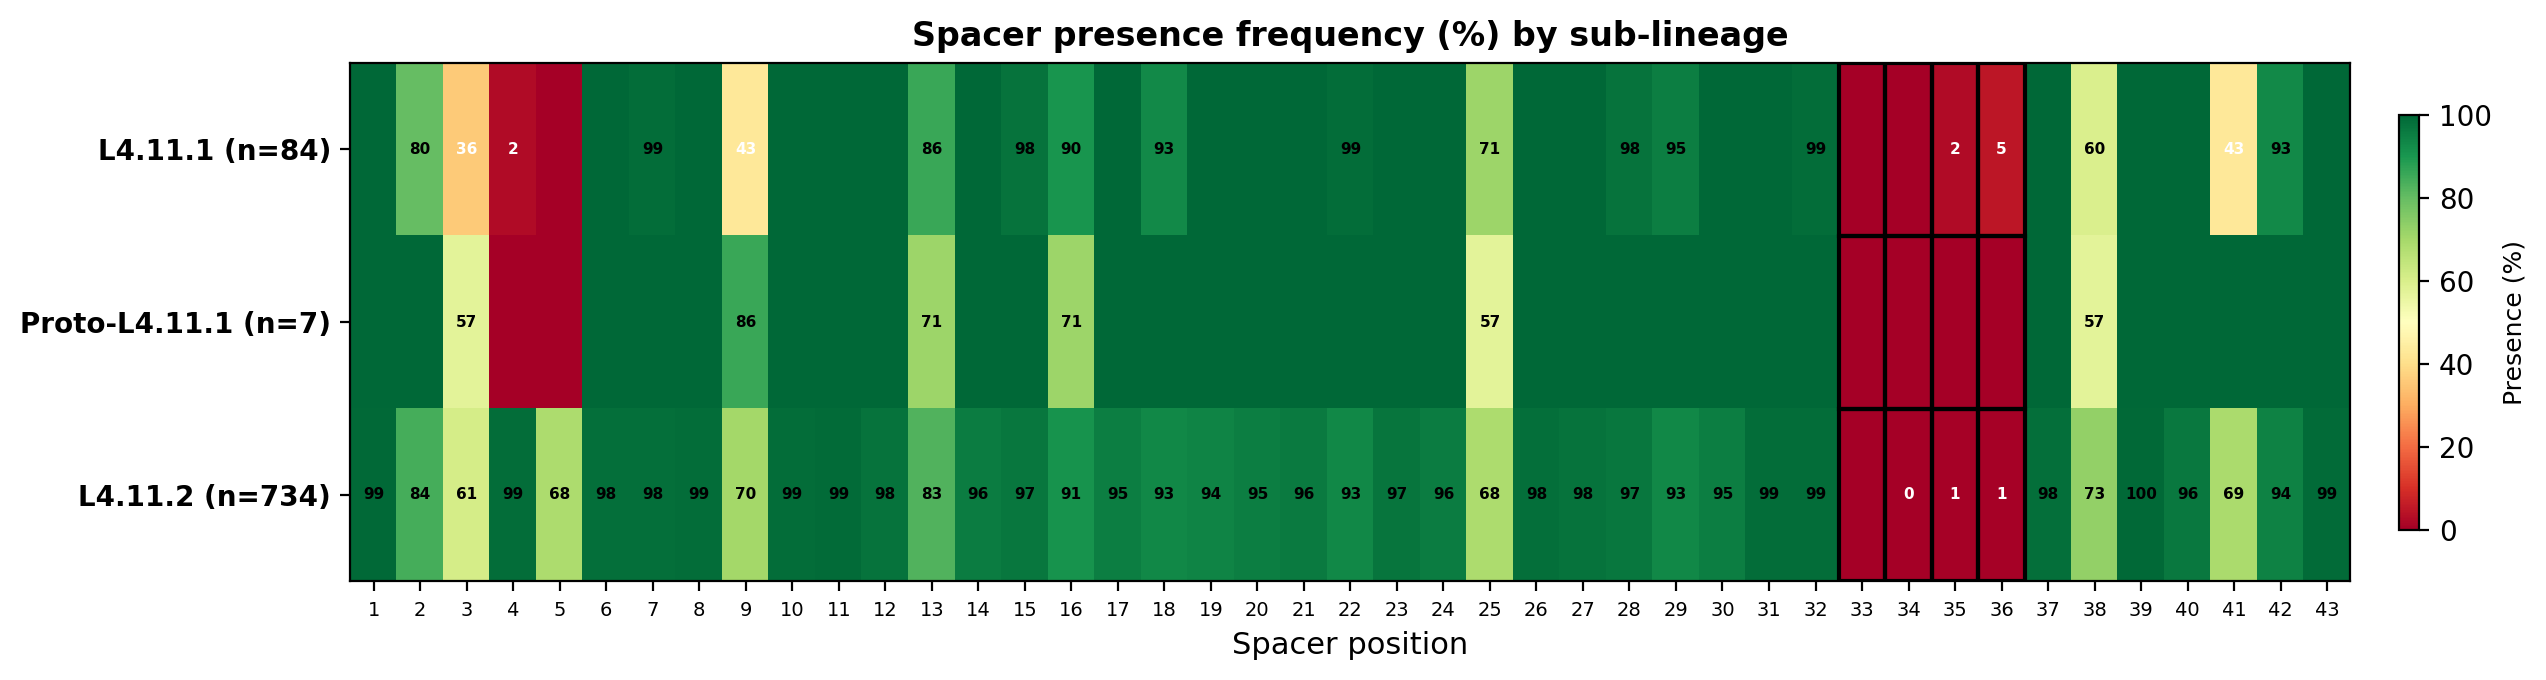
\includegraphics[width=0.9\textwidth]{figures/spoligotype_analysis.png}
	\caption{\textit{In silico} spoligotype analysis of \lignee{L4.11}
		sub-lineages.
		Spacer presence frequency (\%) across the
		43~CRISPR spacers for \lignee{L4.11.1} ($n = 84$),
		Proto-\lignee{L4.11.1} ($n = 7$), and \lignee{L4.11.2} ($n = 734$).
		Red = absent in $>$95\% of SRAs; green = present in $>$95\%.
		Black rectangles highlight spacers 33--36, consistently deleted
		across all sub-lineages (T1 signature).
		Note the differential presence of spacers 3--5 between sub-lineages.}
	\label{fig:spoligo}
\end{figure}
\
\subsection{L4.11 evolutionary context regarding Sreevatsan \textit{et al.} Principal Genetic Grouping (PGG) classification}

The gyrA-katG allelic combination at H37Rv genomic positions 7585 and 2154724 respectively, allows to classify MTBC into three Principal Genetic Groups (PGG)\cite{sreevatsan1997,filliol2006}. It is interesting to note that depending on epidemic clusters, L4.11 may belong to PGG2 or to PGG3, contrarily to the L4.9 that only belongs to PGG3.

\subsection{Drug resistance}

Drug resistance data reveal markedly different profiles between the  two L4.11
sublineages.  Across all 825~\lignee{L4.11} SRAs with variant
reports, 278~(33.8\%) are multidrug-resistant (MDR; resistant to both
isoniazid and rifampicin).  This rate is an order of magnitude higher
than the global  due to bias in sequencing (most sequencing studies are done on MDR-TB) (\textasciitilde3.3\%, WHO 2024~\cite{who2024}).

\lignee{L4.11.1} carries an exceptionally high MDR burden: 78 of
91~SRAs (85.7\%) are MDR\@.  \lignee{L4.11.2}, though more moderate,
still has a high reported MDR rate of 27.4\% (200/731), considerably above the global
average. However these rates do not inform us about the relative epidemic due to the L4.11 lineage as compared to other locally circulating lineages. 

\paragraph{Co-resistance patterns.}

The association between sub-lineage and resistance is statistically
significant for all four first-line drugs (Fisher exact test):
isoniazid (OR\,$=$\,15.7, $p < 10^{-22}$),
rifampicin (OR\,$=$\,9.8, $p < 10^{-19}$),
ethambutol (OR\,$=$\,2.0, $p = 0.002$),
and pyrazinamide (OR\,$=$\,2.3, $p < 10^{-3}$).
Pairwise co-resistance analysis (Figure~\ref{fig:coresist}) reveals that
INH and RIF resistance co-occur almost systematically in \lignee{L4.11.1}
(Jaccard similarity $= 0.94$), consistent with a lineage-fixed MDR
genotype, whereas \lignee{L4.11.2} shows a lower but still substantial
co-occurrence (Jaccard $= 0.65$), indicating independent acquisition
events.  In \lignee{L4.11.1}, 91.2\% (83/91) of SRAs are INH-resistant,
and virtually every INH-resistant strain is also RIF-resistant,
suggesting a clonal MDR genotype rather than sequential accumulation.

\begin{figure}[htbp!]
	\centering
	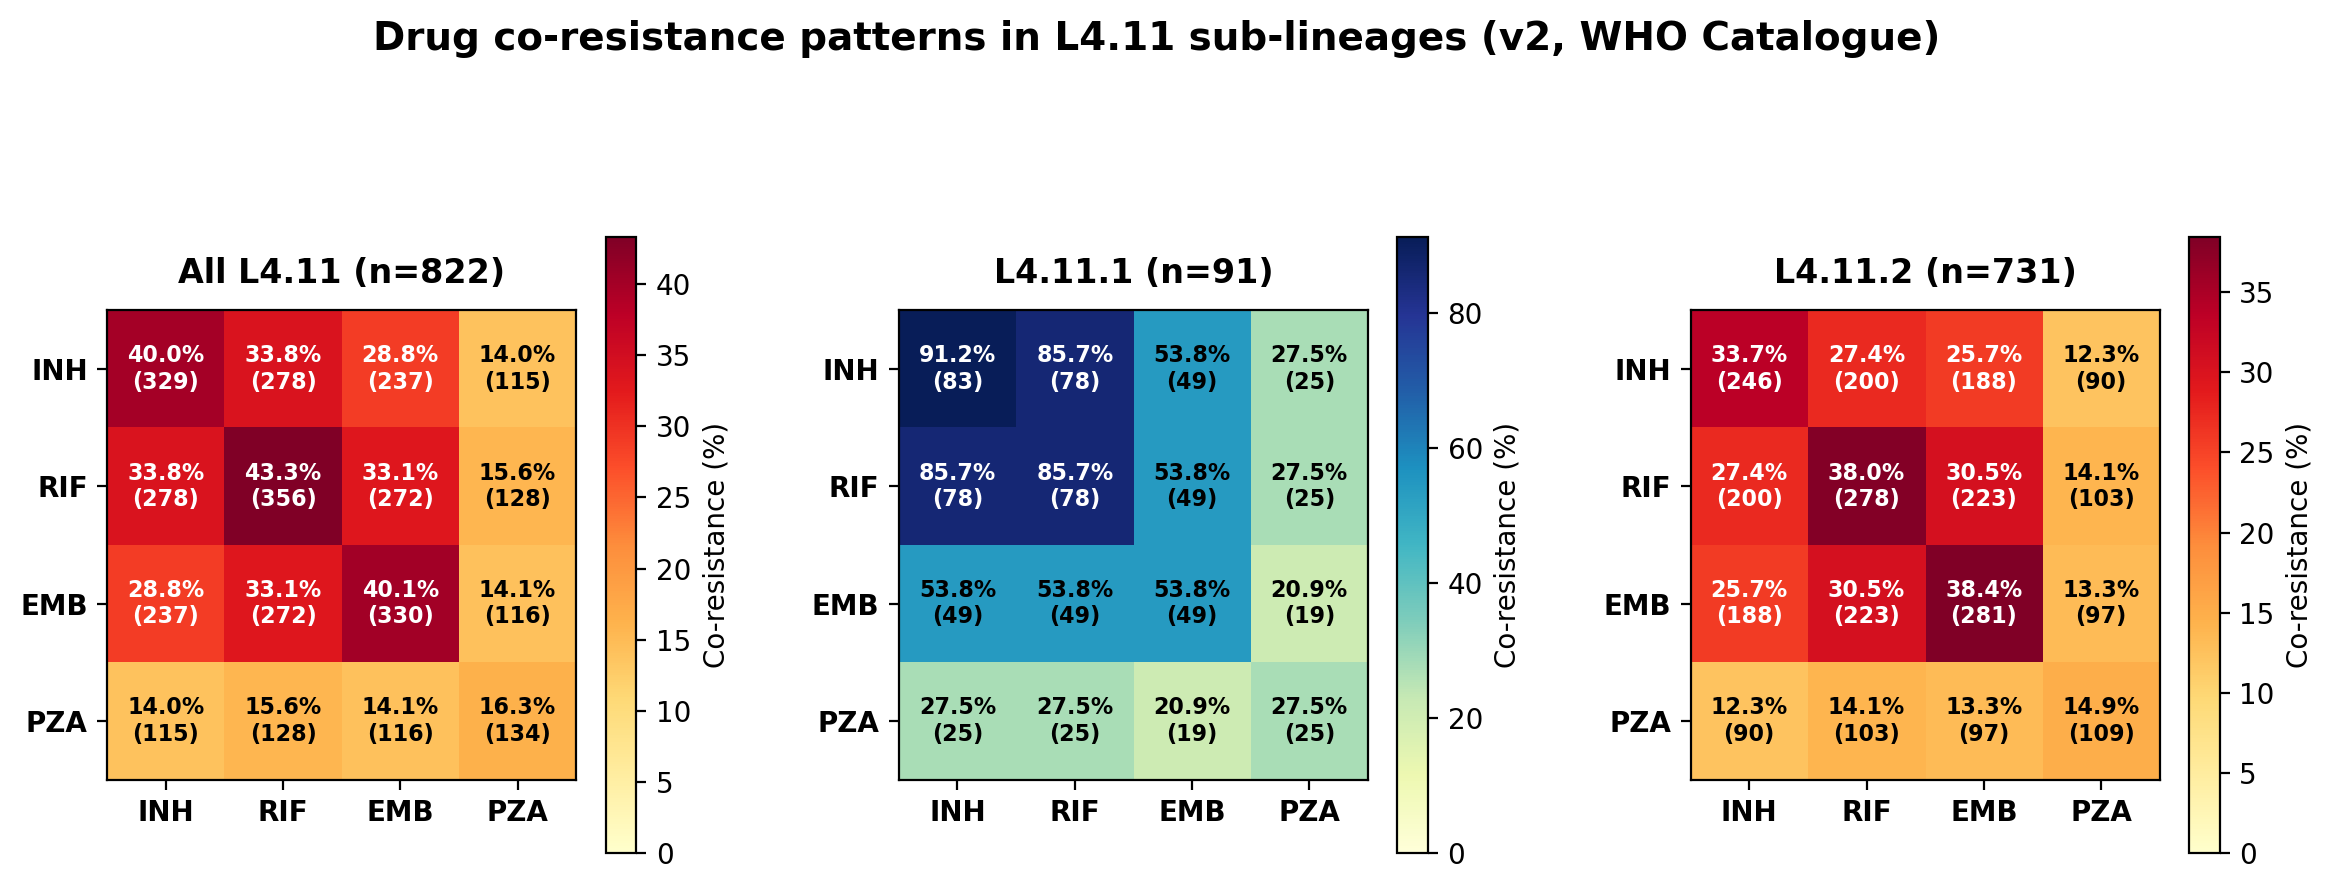
\includegraphics[width=0.85\textwidth]{figures/coresistance_heatmap.png}
	\caption{Drug co-resistance heatmaps for \lignee{L4.11} sub-lineages.
		Each cell shows the percentage (and count) of SRAs
		co-resistant to the corresponding drug pair.
		Diagonal cells indicate single-drug resistance prevalence.
		\textbf{Left:}~All 825~SRAs.
		\textbf{Centre:}~\lignee{L4.11.1} ($n = 91$; blue scale).
		\textbf{Right:}~\lignee{L4.11.2} ($n = 731$; red scale).
		Note the near-saturation of the INH--RIF block in \lignee{L4.11.1},
		consistent with a lineage-fixed MDR genotype.}
	\label{fig:coresist}
\end{figure}
\FloatBarrier

\paragraph{Extended resistance landscape (WHO Catalogue v2).}

By cross-referencing the 825~SRAs against the
WHO Catalogue of mutations associated with drug resistance (2nd~edition,
2023;~\cite{who2023catalogue}), we extended resistance prediction to all
15~anti-TB medicines assessed (Figure~\ref{fig:who_resist}).
Beyond first-line drugs, \lignee{L4.11.1} exhibits a near-fixed
streptomycin resistance (89.0\%, 81/91, mediated predominantly by
\textit{rpsL}~K43R) and emergent fluoroquinolone resistance (11.0\%
levofloxacin/moxifloxacin, via \textit{gyrA}~A90V and S91P).
No WHO-graded resistance-associated mutations were detected for bedaquiline,
clofazimine, delamanid, linezolid, or the injectable aminoglycosides
(kanamycin, amikacin, capreomycin) in either sub-lineage ---
indicating that these agents retain full genotypic activity against
\lignee{L4.11} according to the WHO Catalogue~v2 (however, see
Section~\ref{sec:structural} and the Discussion for the
\textit{mmpR5}~Ile67fs variant and its epistatic context).

\begin{figure}[htbp!]
	\centering
	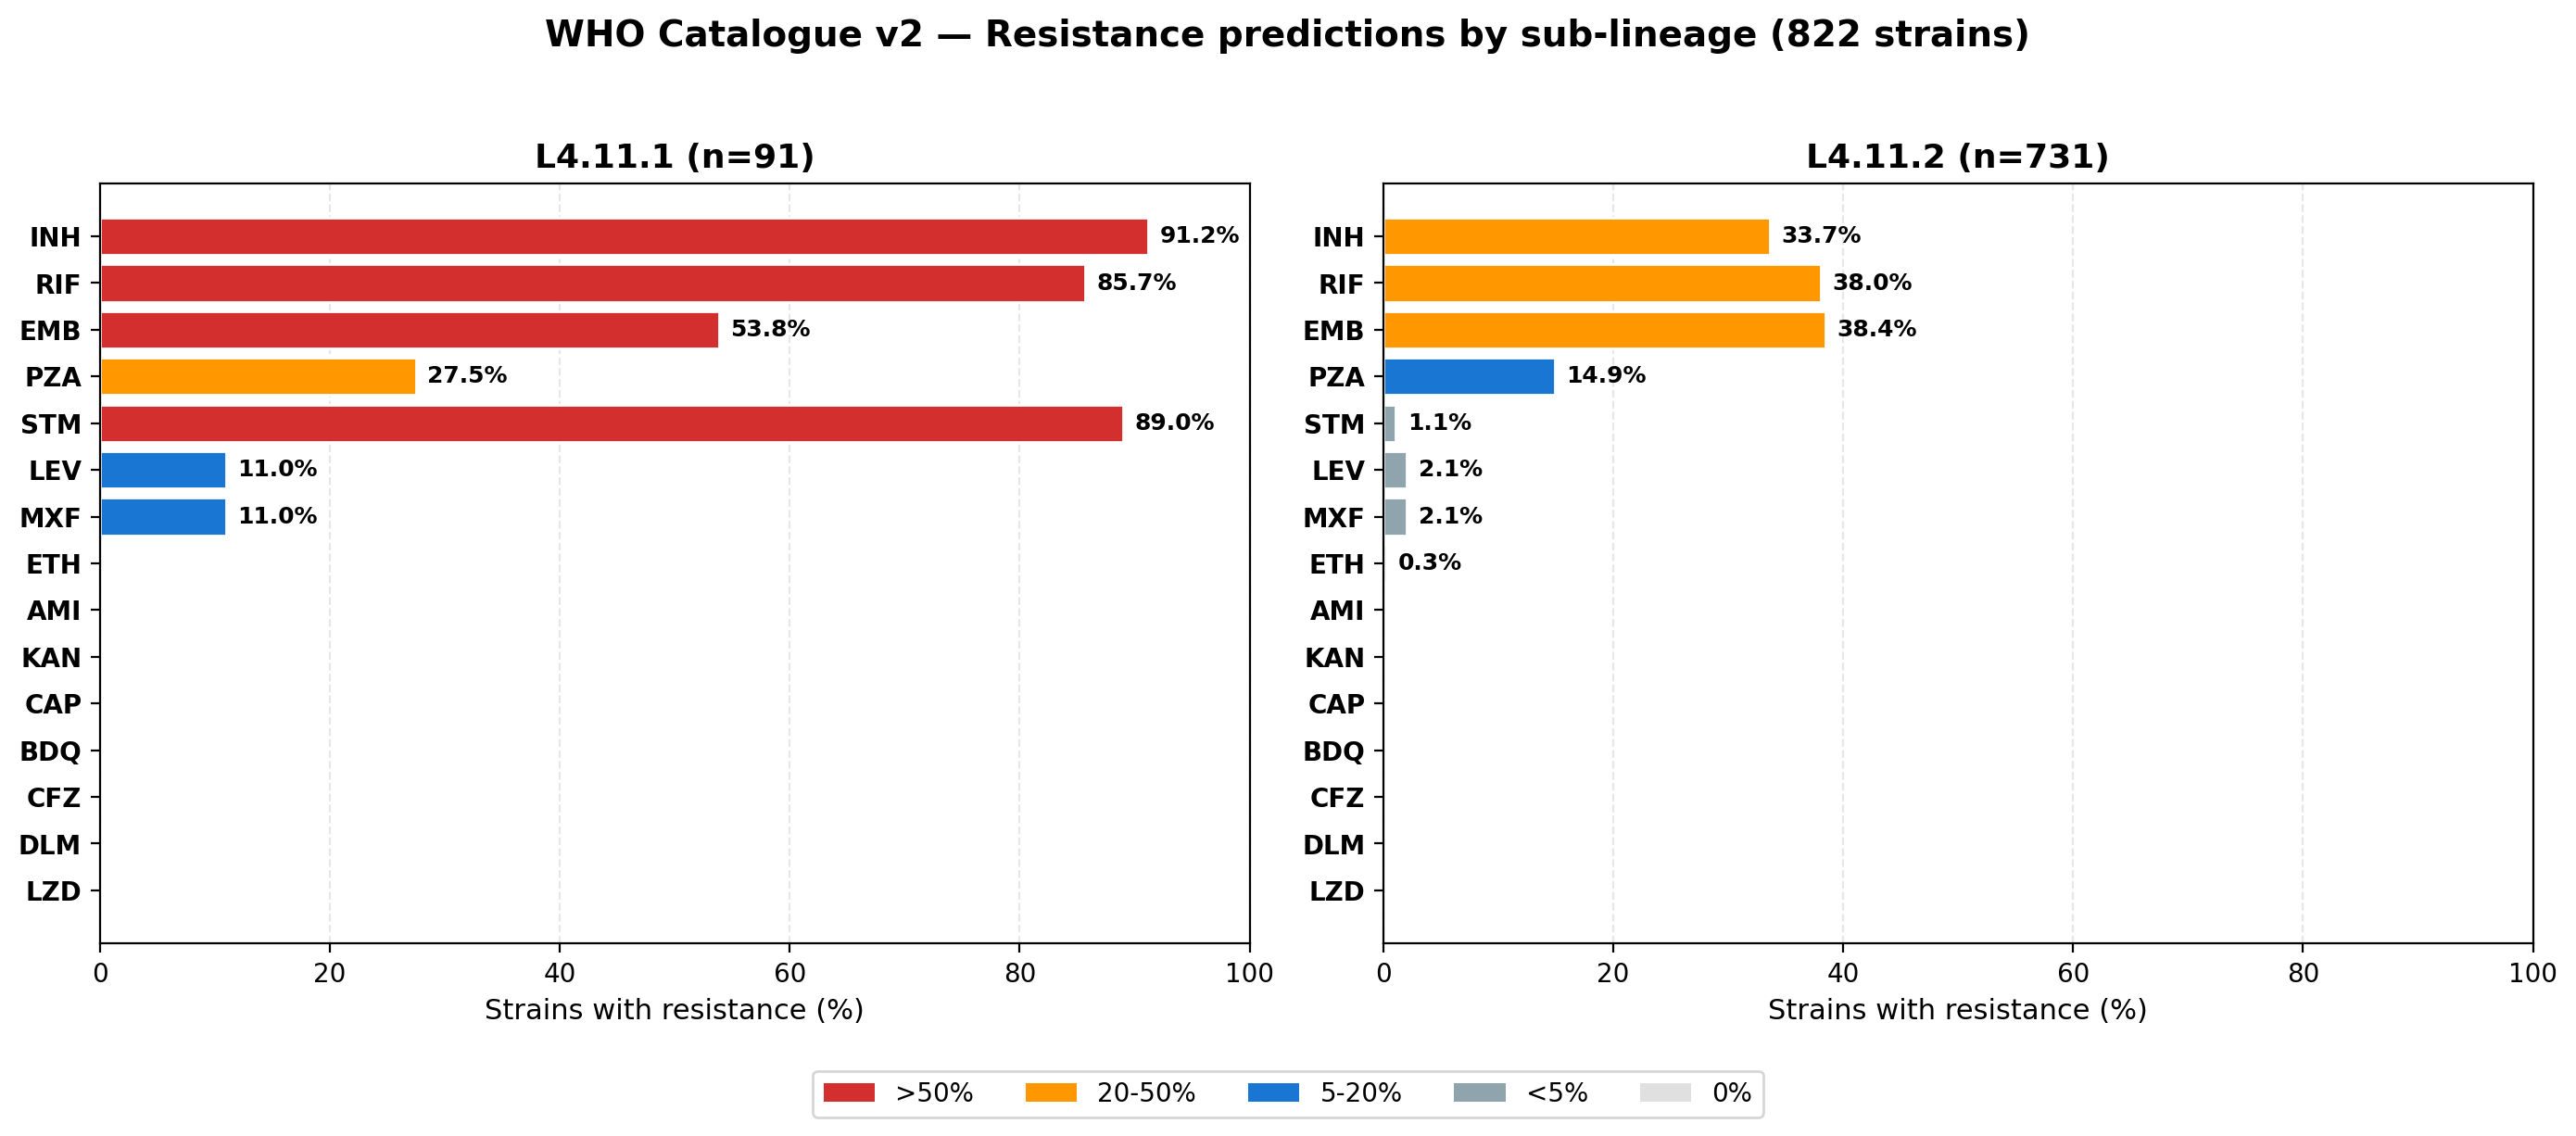
\includegraphics[width=0.75\textwidth]{figures/who_resistance_heatmap.png}
	\caption{WHO Catalogue~v2 resistance predictions for \lignee{L4.11}
		sub-lineages (825~SRAs).
		Bars show the percentage of SRAs carrying at least one
		WHO-graded resistance-associated mutation (R~or~F) per drug.
		\textbf{Left:}~\lignee{L4.11.1} ($n = 91$).
		\textbf{Right:}~\lignee{L4.11.2} ($n = 731$).
		Colours: red, $>$50\%; orange, 20--50\%; blue, 5--20\%; grey, $<$5\%.}
	\label{fig:who_resist}
\end{figure}
\FloatBarrier
Across \lignee{L4.11.2}, 281~SRAs (38.4\%, 281/731) are EMB-resistant --- a rate
comparable to rifampicin resistance (38.0\%).  Strikingly, 40~\lignee{L4.11.2} SRAs
(5.5\%, 40/731) are resistant to EMB \textit{without} concomitant INH or RIF
resistance, an atypical pattern since EMB resistance is conventionally
acquired \textit{after} first-line drug resistance.

To investigate this pattern, we analysed \textit{embB} mutations across
825~\lignee{L4.11} SRAs.  Codon~406
of \textit{embB} emerged as a resistance hotspot specific to
\lignee{L4.11.2}: the G406S substitution is present in 80~SRAs
(all \lignee{L4.11.2}, 10.9\%), while
G406D and G406A account for 30 and 11~additional EMB-R SRAs,
respectively.  The canonical M306I mutation was found in 123~SRAs
(15.0\%).  Notably, 18 of the 40~EMB-only resistant SRAs
carry no known \textit{embB}, \textit{embC}, \textit{embA}, or
\textit{ubiA} mutation.  This observation should be interpreted with
caution: the EMB resistance predictions are genotypic and have not been
confirmed by MIC testing; some of these 18~SRAs may harbour
unrecognised resistance determinants or represent false-positive
predictions.  Nevertheless, the hypothesis that lineage-fixed
cell-envelope perturbations (\textit{pimE}~G53S, \textit{fadE24},
\textit{alkB}~W379R) may confer low-level intrinsic EMB resistance
remains plausible and testable through phenotypic characterisation~\cite{safi2018}.

Additionally, the synonymous mutation \textit{embC}~R927R
(\spdi{4243660:G:A}) is present in $>$97\% of SRAs analysed,
effectively constituting a \textit{de facto} seventh lineage marker
for \lignee{L4.11}.

A comprehensive analysis of drug-resistance gene mutations across
825~SRAs reveals sharply divergent resistance trajectories between the
two sub-lineages.  Isoniazid resistance in \lignee{L4.11.1} is
exclusively mediated by \textit{katG}~S315T~\cite{vilcheze2014}
(91.2\%, 83/91), whereas
\lignee{L4.11.2} relies on \textit{katG}~S315T in only 32\% of SRAs,
with additional rare variants (S315N, G121S, Y413H, A713P) and virtually
no \textit{inhA} promoter mutations.  Each sub-lineage also carries
a lineage-specific non-synonymous \textit{nat} (arylamine
\textit{N}-acetyltransferase) mutation: G78D in \lignee{L4.11.1}
(92.3\%, 84/91) and D27N in \lignee{L4.11.2} (40.9\%, 299/731).

\lignee{L4.11.1} carries a lineage-fixed \textit{panD}~D109N mutation
(100\%, 91/91) ---
the pyrazinoic acid target --- along with \textit{rpsL}~K43R (89.0\%,
81/91), the canonical streptomycin resistance marker.  These mutations
are absent from \lignee{L4.11.2}.

Conversely, \lignee{L4.11.2} harbours a striking bedaquiline/clofazimine
genotype: 24.2\% of SRAs (177/731) carry both the \textit{mmpR5}
(\textit{Rv0678}) frameshift Ile67fs --- a known bedaquiline
resistance-associated variant (RAV) when present in isolation~\cite{andries2014} --- and the
\textit{mmpL5} frameshift Arg202fs (176/731, 24.1\%), which introduces
a premature stop codon at amino acid~206 and abrogates the MmpL5 efflux
pump.
Crucially, this epistatic interaction \textit{reverses} the
resistance-conferring effect of Ile67fs: loss of function of MmpL5
negates the pump overexpression caused by MmpR5 loss of function,
resulting in a \textbf{hypersusceptible} phenotype
(MIC~$<$\,0.12~$\mu$g/mL in 90.9\% of tested isolates)~\cite{nimmo2024}.
Nimmo~et~al.\ estimate this Ile67fs mutation to have emerged around
1702~CE (95\%~CI 1657--1732) in what they term the ``Peruvian clade'',
which corresponds to a subset of our \lignee{L4.11.2}.
These SRAs therefore carry a \textit{de facto} pre-antibiotic-era
mmpR5 variant whose resistant phenotype is silenced by the co-occurring
mmpL5 frameshift, underscoring the importance of considering epistatic
interactions when predicting bedaquiline susceptibility from genomic
data~\cite{nimmo2024,vargas2023}.

Rifampicin resistance is remarkably prevalent: RRDR mutations occur in
85.7\% (78/91) of \lignee{L4.11.1} and 38.0\% (278/731) of
\lignee{L4.11.2}, yielding 356~RRDR-positive SRAs overall (43.3\%).
The dominant RRDR mutation is \textit{rpoB}~S450L (61.5\% L4.11.1,
27.2\% L4.11.2), followed by D435Y (6.0\% L4.11.2) and D435V (1.8\%).
\lignee{L4.11.2} also carries a lineage-fixed synonymous variant V695L
(100\%).

Among the 356~RRDR SRAs, compensatory \textit{rpoC} mutations are
frequent.  The most common is V483G (31~SRAs, all \lignee{L4.11.2}),
followed by L527V (8), and other variants.
\lignee{L4.11.1} exhibits a distinct compensatory path centred on
\textit{rpoC}~Q435P (10/91 SRAs, 11.0\%), a mutation not previously
described in the literature.  Three \lignee{L4.11.2}
SRAs additionally carry \textit{rpoA}~V183A.
The higher compensatory mutation rate in \lignee{L4.11.2} suggests
greater selective pressure for fitness restoration in the Peruvian
population.

\subsection{Genomic structural variation}
\label{sec:structural}

\textit{In silico} IS6110 fingerprinting reveals that both sub-lineages
carry a high IS6110 copy number, with an overall median of 10~copies.
\lignee{L4.11.1} displays a bimodal distribution (range: 2--12, median
10): SRAs from the Bangladeshi BioProject PRJEB38938 carry 2--4~copies,
while SRAs from other BioProjects carry 9--12~copies.
\lignee{L4.11.2} shows a more homogeneous profile (range: 6--17, median
10).  All other insertion sequences (IS1081, IS1557, IS1547,
\textit{etc.}) are strictly conserved between the two sub-lineages
(e.g.\ IS1081: exactly 6~copies in both).

Three IS6110 insertion positions are exclusive to \lignee{L4.11.2} and
absent from \lignee{L4.11.1}:
\begin{sloppypar}
\begin{itemize}
	\item Position 1\,960\,285 ($>$99\%): disrupts the DosR dormancy
	      regulon genes \textit{Rv1733c}--\textit{Rv1735c} and the non-coding RNA
	      \textit{MTS1338}, a key small RNA up-regulated during hypoxia and
	      macrophage infection;
	\item Position 2\,038\,789 ($>$97\%): disrupts the PPE-family
	      protein \textit{PPE28} (Rv1800) and lipoprotein \textit{lppT} (Rv1799);
	\item Position 3\,549\,142 ($>$95\%): disrupts the
	      \textit{vapC45}/\textit{vapB45} toxin--antitoxin system
	      (Rv3180c/Rv3181c), regulating persistence and
	      antibiotic tolerance.
\end{itemize}
\end{sloppypar}
Conversely, a single insertion at position 1\,543\,432 is specific to
\lignee{L4.11.1} ($>$50\%), disrupting the membrane protein Rv1371.
Orientation analysis of the 5\,660~novel IS6110 copies reveals that all
insertions occur in the reverse orientation, with perfect consistency
across all 161~unique insertion sites (no position exhibits mixed
orientations).  This uniformity implies a single transposition mechanism
and argues against independent convergent insertions at the same loci.
Two ancestral insertion sites (positions 1\,987\,702 and 3\,120\,522) are
shared by both sub-lineages; the former disrupts the cutinase \textit{cut1}
(Rv1758), a lipolytic enzyme involved in cell-envelope remodelling.

\paragraph{Gene deletions.}

Analysis of genes with insufficient coverage (potential deletions) across
all 825~SRAs reveals lineage-specific deletion
blocks.

A contiguous block of four genes (Rv1758--Rv1762c) is deleted in
virtually all \lignee{L4.11.2} SRAs: \textit{cut1} (cutinase, 100\%),
Rv1760 (diacylglycerol acyltransferase, 100\%), Rv1761c and Rv1762c
(99\%).  This deletion corresponds precisely to the ancestral IS6110
insertion at position 1\,987\,702 shared by both sub-lineages, suggesting
that the IS6110 at this locus triggered a secondary deletion in
\lignee{L4.11.2} that extended to neighbouring genes.  Notably, Rv1760
catalyses the terminal step of triacylglycerol (TAG) biosynthesis;
its loss deprives \lignee{L4.11.2} of a key lipid storage pathway.

A second deletion block (Rv0573c--Rv0574c) affects 31\% of
\lignee{L4.11.2}: \textit{pncB2} (nicotinic acid
phosphoribosyltransferase), involved in the NAD$^+$ salvage pathway.
A third block comprising \textit{PPE58} and two transposases
(Rv3426--Rv3428c) is deleted in 29\% of \lignee{L4.11.2} SRAs.

\lignee{L4.11.1} carries a distinct deletion signature.
Twelve phage-protein genes (Rv1573--Rv1586c, prophage PhiRv1) are
deleted in 100\% of \lignee{L4.11.1} but only 2\% of \lignee{L4.11.2},
indicating prophage excision specific to this sub-lineage.  Additionally,
the toxin \textit{vapC25} (Rv0277c) is deleted in 72\% of
\lignee{L4.11.1} SRAs --- a second toxin--antitoxin perturbation
alongside the \textit{vapC45} IS6110 disruption observed in
\lignee{L4.11.2}.
No gene exhibited a coverage ratio $\geq$\,2$\times$ the genome-wide
median in a majority of SRAs of either sub-lineage, indicating
that the structural variation landscape of \lignee{L4.11} is dominated
by deletions and IS6110 insertions rather than segmental duplications.

\paragraph{RD-typing validation.}

\textit{In silico} RD-typing confirms the phylogenetic coherence of
\lignee{L4.11}.  All 78~canonical Regions of Difference (RD105--RD761)
are intact in both sub-lineages, consistent with a standard Lineage~4
profile.  Two deletions define the lineage as a whole: RD715
(100\%, 825/825) and the 7-bp deletion in \textit{pks15/1} (100\%),
accompanied by 11~shared custom genomic segments absent in 96--100\% of
all SRAs.

A single large deletion at position 1\,779\,266--1\,788\,513
($\sim$9.2~kb, prophage PhiRv1) is present in 100\% of
\lignee{L4.11.1} (91/91) but only 3.3\% of \lignee{L4.11.2}
(24/731).  This region carries three overlapping catalogue
entries --- DS5, RD3, and ``149'' --- which represent nomenclature
variants from different classification schemes rather than
independent deletions.  The PhiRv1 deletion provides a robust
RD-based marker for sub-lineage discrimination.  Conversely, the genomic
segment at position 3\,549\,142--3\,554\,067 is deleted in 95\% of
\lignee{L4.11.2} but only 2\% of \lignee{L4.11.1},
corresponding to the IS6110-mediated disruption of the
\textit{vapC45}/\textit{vapB45} toxin--antitoxin locus.

Profile diversity reflects the IS6110 expansion: \lignee{L4.11.1} has
28~unique RD profiles among 91~SRAs, whereas \lignee{L4.11.2}
exhibits $>$300~unique profiles among 731~SRAs.

\subsection{Virulence-associated mutations and selection pressure}

We systematically screened all non-synonymous variants in virulence gene
families (PE/PPE, \textit{mce}, ESX/Type~VII, DosR regulon, lipid metabolism,
toxin--antitoxin systems, sigma factors, and two-component regulators)
across all 825~SRAs.

\paragraph{PE/PPE family.}
Twelve PE/PPE mutations are fixed ($>$90\%) in both sub-lineages,
including a stop-gain in \textit{PE35} (E99*, 100\%), which
abolishes the ESAT-6-adjacent protein involved in ESX-1 secretion.
Four additional PPE mutations are L4.11.2-specific ($>$96\%): \textit{PPE33}
G300E, \textit{PPE64} N196Y, \textit{PPE25} G191R, and \textit{PPE56} V203G.

\paragraph{\textit{mce} operons.}
Three \textit{mce} mutations are shared (\textit{mce1F} L370P, \textit{mce2A} F51S, \textit{mce3F} A396E).
\lignee{L4.11.1} carries three exclusive \textit{mce} mutations: \textit{mce1C} G340V,
\textit{mce2F} G391fs (frameshift disrupting the cholesterol uptake
operon), and \textit{mce4F} F541P.  \lignee{L4.11.2} has \textit{mce1D} V410A (100\%).

\paragraph{ESX/Type~VII secretion.}
Five ESX mutations are shared ($>$99\%), including \textit{eccC3} P214R and
\textit{espA} T192I.  \lignee{L4.11.2} has five specific ESX mutations,
notably \textit{esxL} S39G (98\%) and \textit{eccCa1}/\textit{eccCb1} variants in ESX-1.
\lignee{L4.11.1} carries \textit{eccC2} A990T (100\%).

\paragraph{Lipid metabolism.}
This category shows the most striking lineage-specific differentiation.
Ten mutations are shared ($>$97\%), including \textit{fadE24} P130L, \textit{mmpL2} R426H,
and variants in \textit{pks2}, \textit{pks8}, \textit{pks12}, and \textit{pks15}.  \lignee{L4.11.1} carries
eight exclusive mutations: \textit{pks6} V1146A, \textit{fadE12} K138M,
\textit{fadD25} I353fs (frameshift), \textit{pks8} P715A, \textit{mmpL9} G928R,
\textit{pks2} G9V, \textit{pks6} G51V, and \textit{fadD29} M618T.  \lignee{L4.11.2} has five
exclusive lipid mutations, including a second hit in \textit{fadE24}
(I116L, 100\%) alongside \textit{fadD1} P517L, \textit{fadE5} T71P, and \textit{fadD26} Q163R.

\paragraph{Regulatory systems.}
Two sigma factors carry shared frameshift mutations:
\textit{sigI} S278fs (99.5\%) and \textit{sigM} R160fs (93--100\%),
indicating loss of two alternative sigma factors in the entire lineage.
In the DosR dormancy regulon, \lignee{L4.11.1} carries
\textit{devS} K509E (100\%) and \textit{narK3} G137D (100\%), altering both the
sensor kinase and the nitrate transporter of the dormancy response.

\paragraph{Toxin--antitoxin systems.}
Two TA mutations are shared (\textit{vapB22} A56V, \textit{vapC47} S46L).
\lignee{L4.11.1} carries \textit{vapC29} T33I and \textit{mazF6} A41V (100\%),
adding a toxin perturbation to the \textit{vapC25} deletion observed in this
sub-lineage.

These mutations reveal a lineage undergoing extensive functional
diversification, with \lignee{L4.11.1} accumulating disruptions in lipid
metabolism and dormancy pathways, while \lignee{L4.11.2} diverges in
ESX secretion and cell-envelope modification.

\subsection{Transmission clustering}

Pairwise SNP distances were computed across all 825~SRAs using the
symmetric difference of SPDI variant sets.  Because all SRAs were
called against the same reference (\spdi{NC\_000962.3}) with an identical
pipeline, the symmetric SPDI set difference is functionally equivalent to
a core-genome SNP distance; each SPDI corresponds to a single nucleotide
variant at a defined genomic position, and the symmetric difference
counts the number of sites at which two SRAs differ.  At a threshold of
$<$12~SNPs --- widely used for recent transmission in
\textit{M.\,tuberculosis}~\cite{walker2013} --- 138~pairs were identified, grouping
226~SRAs (27.4\%) into 105~clusters by single-linkage.

The clustering rate differed markedly between sub-lineages:
\lignee{L4.11.2} showed 29.7\% (217/731$+$3 basal) of SRAs in clusters,
compared with 9.9\% (9/91) for \lignee{L4.11.1}.  No cross-lineage
pair was detected below the 12-SNP threshold, confirming the complete
epidemiological separation of the two sub-lineages.

The three largest clusters comprised 6, 5, and 5~SRAs respectively.
Two belonged to \lignee{L4.11.2} (CRyPTIC isolates, predominantly
Peruvian), while the third consisted of five \lignee{L4.11.1}
Bangladeshi isolates from the same BioProject (SRR35281596--602).
Among the 101~pairs with $\leq$4~SNPs, the majority (94\%) involved
\lignee{L4.11.2}, suggesting ongoing chains of recent transmission in
Peru.  The overall distance distribution was dominated by pairs
$\geq$100~SNPs (90.3\%), consistent with the deep divergence between
the two geographic foci of L4.11.

Because the SPDI set-difference metric has not been independently
calibrated against core-genome SNP distances, we performed a
sensitivity analysis at seven distance thresholds
(Table~\ref{tab:clustering_sensitivity}).  The clustering rate
increases monotonically from 20.5\% ($<$2~SPDI) to 61.3\% ($<$30~SPDI),
with the 12-SPDI threshold yielding results within the range typically
reported for \textit{M.\,tuberculosis} populations.  Across all
thresholds, \lignee{L4.11.2} consistently shows a higher clustering
rate than \lignee{L4.11.1}, confirming that this difference is robust
to threshold choice.

\begin{table}[htbp!]
	\centering
	\small
	\caption{Sensitivity analysis of transmission clustering at different
		SPDI-distance thresholds.  Clustering defined by single-linkage.
		Percentages computed over $n = 825$ (All), $n = 91$ (L4.11.1),
		and $n = 734$ (L4.11.2 including 3~basal SRAs).}
	\label{tab:clustering_sensitivity}
	\begin{tabular}{rrrrrr}
		\toprule
		\textbf{Threshold} & \textbf{Pairs} & \textbf{Clustered} & \textbf{\% All} & \textbf{\% L4.11.1} & \textbf{\% L4.11.2} \\
		\midrule
		$<$2   &  89 & 169 & 20.5 &  4.4 & 22.6 \\
		$<$5   & 101 & 193 & 23.4 &  6.6 & 25.6 \\
		$<$8   & 105 & 200 & 24.2 &  7.7 & 26.4 \\
		\textbf{$<$12} & \textbf{138} & \textbf{226} & \textbf{27.4} & \textbf{9.9} & \textbf{29.7} \\
		$<$15  & 191 & 264 & 32.0 & 12.1 & 34.6 \\
		$<$20  & 338 & 337 & 40.8 & 17.6 & 43.9 \\
		$<$30  & 1062 & 506 & 61.3 & 46.2 & 63.5 \\
		\bottomrule
	\end{tabular}
\end{table}

\paragraph{Selection pressure across gene families.}

To assess selective constraints, we computed the ratio of unique
non-synonymous ($p_N$) to synonymous ($p_S$) variant sites per gene
across all 825~SRAs (2{,}966~genes;
5{,}537~non-synonymous and 2{,}757~synonymous sites).

The genome-wide $p_N/p_S$ ratio is 2.00 overall, 2.17 for
\lignee{L4.11.1} and 1.97 for \lignee{L4.11.2}.  The slightly elevated
ratio in \lignee{L4.11.1} is consistent with a recent population
bottleneck.  Because the site-based $p_N/p_S$ metric used here is
inherently inflated in recently diverged clonal populations (see
Section~\ref{sec:methods}), a genome-wide value $>1$ is expected under
neutral drift with small effective population size and does not, by
itself, demonstrate positive selection.  To assess whether individual
gene families show a statistically significant non-synonymous excess
relative to the genome-wide baseline, we applied Fisher exact tests
on $2 \times 2$ contingency tables ($p_N$/$p_S$ counts per category
vs.\ all remaining genes; Bonferroni-corrected for five comparisons).

Among virulence gene families, drug-resistance targets show the highest
aggregate $p_N/p_S$ (11.4; 183~$p_N$, 16~$p_S$; Fisher OR $= 5.86$,
$p_{\mathrm{Bonf}} < 10^{-16}$), driven by
\textit{pncA} (39/0), \textit{katG} (23/0), and \textit{rpoB}
(47/6).  This is the only gene family significantly enriched in
non-synonymous variants relative to the genomic background.
Sigma factors also show a marked non-synonymous excess
($p_N/p_S = 2.8$), reflecting the \textit{sigI} and \textit{sigM}
frameshifts fixed in L4.11.
Lipid metabolism genes maintain $p_N/p_S = 2.0$ (298/149; Fisher
$p = 0.96$, NS) with notable
outliers: \textit{fadE24} (5/0), \textit{fadD23} (6/0), \textit{pks6}
(8/1), and \textit{pks7} (9/2).  In contrast, \textit{fadD32} --- encoding
an essential mycolic acid synthase --- is under strong purifying
selection (0/5, $p_N/p_S = 0$), confirming its indispensability.
The ESX/Type~VII secretion family shows $p_N/p_S = 1.8$ (145/80;
Fisher $p = 0.47$, NS), with
\textit{espB} (7/0) and \textit{eccC2} (17/6) exhibiting a pronounced
non-synonymous excess at the gene level.

PE/PPE genes display a moderate non-synonymous excess ($p_N/p_S = 1.7$;
471/277; Fisher $p = 0.02$, NS after Bonferroni correction),
but with marked heterogeneity: \textit{PPE13} (11/1) and
\textit{PPE56} (23/8) are strongly enriched in non-synonymous variants, whereas
\textit{PPE34} (4/12, $p_N/p_S = 0.33$) is the most conserved member,
under strong purifying selection.

\paragraph{Homoplastic mutations.}

\begin{sloppypar}
To identify mutations under convergent selective pressure, we screened
for variants present at $>$5\% frequency in \emph{both} sub-lineages
but not fixed ($>$90\%) in both --- a signature of independent emergence
on separate phylogenetic branches.  This analysis identified
106~homoplastic sites, of which 45 are non-synonymous, 26 are
synonymous, and the remainder intergenic.

PE/PPE genes harbour the largest share of non-synonymous homoplasies
(28/45, 62\%).  \textit{PE\_PGRS9} alone carries five convergent
missense variants (e.g.\ Thr445Ala, 79\%/82\% in L4.11.1/L4.11.2),
\textit{PE\_PGRS4} and \textit{PE\_PGRS10} contribute four each, and
\textit{PPE54}~Ala1645fs is nearly fixed in both sub-lineages
(98\%/89\%).  This pattern indicates ongoing functional
diversification of the PE/PPE surface antigen family across independent
evolutionary trajectories, consistent with immune-evasion-driven
selection or relaxed purifying constraint on surface-exposed antigens.
\end{sloppypar}

Drug-resistance mutations also show convergence: \textit{katG}~S315T
(isoniazid) is present at 91\% in \lignee{L4.11.1} and 32\% in
\lignee{L4.11.2}; \textit{rpoB}~S450L (rifampicin) at 62\%/27\%;
\textit{embB}~M306I (ethambutol) at 11\%/10\%; and \textit{gyrA}~S95T
(fluoroquinolone-associated) at 71\%/96\%.  The independent acquisition
of the same canonical resistance mutations in both geographic foci
underscores the convergent evolution of multidrug resistance in L4.11.

Additional convergent loci include \textit{Rv3428c} (three homoplasies
including a frameshift at 100\%/73\%), the serine/threonine phosphatase
\textit{pstP}~P463S (84\%/89\%), and the lipid biosynthesis gene
\textit{ppsA}~R877H (77\%/84\%).

\subsection{Spatio-temporal reconstruction}

Molecular clock analysis with TreeTime estimated the TMRCA of \lignee{L4.11}
to approximately \textbf{1965} (bootstrap 95\% CI: 1560--1996;
Figure~\ref{fig:clock}).
However, the root-to-tip regression on the 143~SRAs with known
collection dates yields $R^2 = 0.008$, indicating a very weak temporal
signal.  The point estimate should therefore be regarded as preliminary.
The root-to-tip regression for \lignee{L4.11.2} displays a positive temporal
trend consistent with clock-like evolution, whereas four
\lignee{L4.11.1} SRAs were identified as clock outliers (apparent
dates $< -3000$), suggesting rate heterogeneity between the two
sub-lineages or long-branch effects from the Bangladesh clade.  These
outliers were excluded from the molecular clock estimation; the remaining
\lignee{L4.11.2} SRAs yielded the best available temporal signal,
but the wide confidence interval (spanning over four centuries)
underscores the need for denser temporal sampling to refine this estimate.

A TreeTime mugration analysis was performed to infer ancestral geographic
states.  However, the inferred root state was highly sensitive to sampling
frequencies (the root was assigned to Peru, which represents 69\% of
geo-localised SRAs), indicating that the mugration model reflects
sampling density rather than true dispersal history. We therefore do not
report mugration-derived corridors and consider the geographic origin of
\lignee{L4.11} as an open question (see Discussion).

\begin{figure}[htbp!]
	\centering
	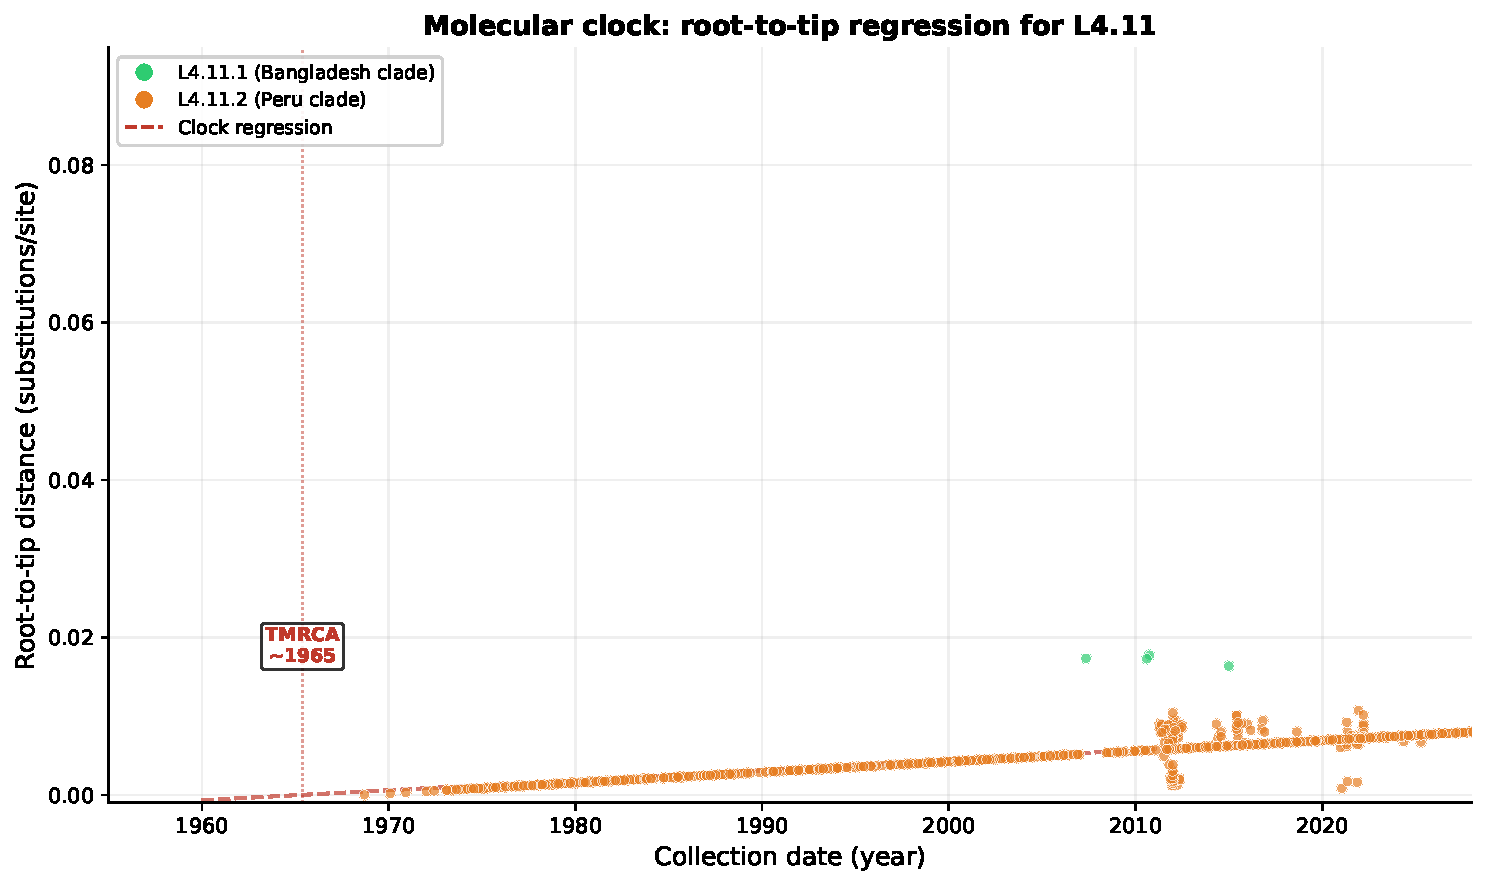
\includegraphics[width=0.6\textwidth]{figures/fig3_molecular_clock.pdf}
	\caption{Root-to-tip regression for \lignee{L4.11} SRAs with known collection
		dates.  Green points: \lignee{L4.11.1} (Bangladesh clade); orange points:
		\lignee{L4.11.2} (Peru clade).  The dashed line indicates the clock
		regression, with the estimated TMRCA around 1965
		(bootstrap 95\% CI: 1560--1996; $R^2 = 0.008$).}
	\label{fig:clock}
\end{figure}
\FloatBarrier


% ── Discussion ───────────────────────────────────────────────────────────────
\section{Discussion}

Our analysis of 825~publicly available \lignee{L4.11} genomes reveals a
lineage with rich internal structure, high drug resistance burden, and a
remarkable phylogeographic partition.

The enrichment from 415 to 825~SRAs yielded important refinements.  Three
additional markers that were core-exclusive in the initial v1 dataset lost
this status upon dataset expansion, while all eight current core-exclusive
markers (Table~\ref{tab:core_excl}) proved robust.  This validates our
iterative approach to marker identification and underscores the importance
of large, independently assembled datasets for defining lineage-specific
barcodes.

The identification of two complementary sub-lineages ---
\lignee{L4.11.1} (91~SRAs, 107~core-exclusive markers) and
\lignee{L4.11.2} (731~SRAs, 16~core-exclusive markers) --- substantially
refines the phylogenetic resolution within this previously undifferentiated
clade.  \lignee{L4.11.1}, with 107~core-exclusive markers, is among the
best-defined novel sub-lineages identified in lineage~4 to date, rivalling
the resolution of entire lineage-level classifications.

The phylogeographic partition between the two sub-lineages is striking.
\lignee{L4.11.2} is overwhelmingly South American (Peru: 80\%), consistent
with the monophyletic MDR cluster from Lima described by
Vargas~et~al.~\cite{vargas2023} in the context of bedaquiline and
clofazimine resistance.  In contrast, \lignee{L4.11.1} is centred on
Bangladesh (81\%) with secondary representation in East Africa (South
Africa, Uganda).

The TreeTime mugration analysis places the most probable geographic
state at the root node as Bangladesh.  However, as noted above, this
result is \emph{not reliable}: \lignee{L4.11.1} and
\lignee{L4.11.2} are phylogenetically \emph{sister clades}, not
ancestor-descendant lineages, and mugration inference is highly sensitive
to sampling density (Peru represents 69\% of geo-localised SRAs).
We report this result for completeness only, and the geographic origin of
the common ancestor of \lignee{L4.11} remains an open question.
The Proto-\lignee{L4.11.1} SRAs
(South Africa, United Kingdom) and the broader IS6110 hotspot analysis
(dominated by Portuguese and South African SRAs) are also consistent
with a European dispersal route.
\lignee{L4.11.2} represents a successful intercontinental dispersal to
South America, where it has undergone substantial diversification and
acquired extensive drug resistance.  The estimated TMRCA of
approximately 1965 (95\% CI: 1560--1996) places the divergence
of this lineage tentatively in the late 20th century,
a timeframe consistent with the global expansion of multidrug-resistant TB\@.
The geographic clustering --- Peru and USA sharing 55~\lignee{L4.11.2}
SRAs, Bangladesh and East Africa sharing \lignee{L4.11.1} --- is
consistent with known migration patterns between these regions and
with historical links between South Asian and African TB epidemics.

The drug resistance profile of \lignee{L4.11} is alarming.  MDR rates
exceed the global average by an order of magnitude, and
\lignee{L4.11.1} carries an extraordinarily high burden.  However,
these rates must be interpreted with caution.  The BioProject composition
of our dataset reveals systematic ascertainment biases:
PRJEB38938 (Bangladesh, 37~SRAs) is an MDR surveillance study,
PRJEB32234 (Peru, 198~SRAs) focuses on drug-resistant lineages,
and PRJNA595834 (Peru, 88~SRAs) targets MDR/XDR isolates from
diabetes-comorbid patients.  Together, these three BioProjects --- all
designed to enrich for resistant SRAs --- contribute 39\% of the
dataset.  The observed MDR rates therefore represent upper-bound estimates
rather than population-level prevalence.  Whether the residual
association between \lignee{L4.11} and drug resistance persists after
correcting for ascertainment bias will require comparison with
population-representative surveillance cohorts.  In particular,
the 86\% MDR rate in \lignee{L4.11.1} likely reflects the composition
of the Bangladeshi MDR study rather than an intrinsic lineage property.
Longitudinal epidemiological studies from both South Asia and South
America are needed to disentangle lineage-specific resistance
acquisition from sampling artefacts.

The \textit{embB} codon~406 hotspot (G406S/D/A) found in 121~\lignee{L4.11.2}
SRAs is particularly noteworthy.  This codon is a recognised
ethambutol resistance determinant, yet its concentration within a single
sub-lineage of \lignee{L4.11} has not been reported.  The presence
of 40~SRAs with EMB resistance \textit{in the absence of} INH or RIF
resistance is atypical, as the classical resistance escalation pathway
begins with INH mono-resistance before progressing to
MDR\@.  The 18~EMB-only resistant SRAs without any canonical
\textit{embB}/\textit{embC}/\textit{ubiA} mutation raise the hypothesis
that lineage-fixed cell-envelope alterations --- particularly
\textit{pimE}~G53S (PIM biosynthesis), \textit{alkB}~W379R (fatty acid
$\omega$-hydroxylation), and the dual \textit{fadE24} perturbation
(mycolic acid recycling) --- may collectively reduce ethambutol
permeability or target accessibility, conferring low-level intrinsic
resistance.  This hypothesis is testable through MIC determination
on a panel of \lignee{L4.11.2} SRAs without \textit{embB} mutations.

The complete mutational profiling of drug-resistance genes confirms that
the two sub-lineages have evolved their resistance independently.
\lignee{L4.11.1} follows a classical MDR trajectory (\textit{katG}~S315T
$\to$ \textit{rpoB} RRDR mutations) supplemented by lineage-fixed
\textit{panD}~D109N and \textit{rpsL}~K43R, conferring intrinsic
pyrazinamide and streptomycin resistance.

\lignee{L4.11.2}, in contrast,
has acquired resistance through a broader mutational spectrum.
The \textit{mmpR5}~Ile67fs + \textit{mmpL5}~Arg202fs genotype found
in 24\% of \lignee{L4.11.2} SRAs merits particular discussion.
Although Ile67fs is classified as a bedaquiline/clofazimine RAV when
considered in isolation, Nimmo~et~al.~\cite{nimmo2024} demonstrated
that the concomitant mmpL5 loss-of-function mutation counteracts
resistance through epistasis, producing a \textbf{hypersusceptible}
phenotype.  Their phylogenetic dating places the emergence of this
Ile67fs variant at approximately 1702~CE (95\%~CI 1657--1732), well
before the antibiotic era, in what they termed the ``Peruvian clade''
--- a clade that overlaps substantially with our \lignee{L4.11.2}.
This finding carries important implications: (i)~genotypic prediction of
bedaquiline resistance from \textit{mmpR5} mutations alone is
insufficient and must jointly consider \textit{mmpL5} status;
(ii)~the 24\% prevalence reflects a historic reservoir of silenced RAVs
rather than active resistance; and (iii)~the loss of a single compensatory
mutant could reactivate bedaquiline resistance in this population,
emphasising the need for phenotypic drug-susceptibility testing.
The predominance of \textit{rpoC}~V483G as a
compensatory mutation in \lignee{L4.11.2} --- a recognised fitness
restorer for \textit{rpoB}~S450L mutants --- further suggests that this
sub-lineage has undergone significant adaptation to maintain
transmissibility despite drug resistance.

The functional annotation of core-exclusive markers reveals a noteworthy
mutational landscape.  At the \lignee{L4.11} level, four of six markers are
non-synonymous: Rv0999~T81A (hypothetical protein), Rv1231c~E171D (membrane
protein), \textit{hisC1}~A23V (histidinol-phosphate aminotransferase~1),
and \textit{fadE24}~P130L (acyl-CoA dehydrogenase, fatty acid $\beta$-oxidation).
The \textit{ethR} intergenic mutation (\spdi{4328316:G:A}) lies in the
regulatory region controlling ethionamide resistance, raising questions about
baseline ethionamide susceptibility in this lineage.

Among the 16~core-exclusive markers of \lignee{L4.11.2}, the \textit{rpoB}
V695L mutation is particularly significant.  This substitution falls within
the $\beta$~subunit of RNA polymerase --- the primary target of rifampicin
--- although codon~695 lies outside the canonical RRDR (codons~426--452).
This lineage-fixed polymorphism in a drug-target gene may modulate the
fitness cost of additional resistance mutations acquired within the RRDR,
potentially facilitating the emergence of rifampicin resistance.  The
\textit{ppk1}~G340C mutation affects polyphosphate kinase, which is required
for Mtb persistence, biofilm formation, and long-term survival in
macrophages.  The \textit{orn}~D70N mutation alters oligoribonuclease, a key
enzyme in RNA turnover and the stringent response.

A striking observation is the dual perturbation of histidine biosynthesis
across the lineage: the \textit{hisC1}~A23V coding mutation defines all
\lignee{L4.11}, while \lignee{L4.11.2} additionally carries an intergenic
mutation near \textit{hisC2} (\spdi{4216744:T:C}).  These two genes encode
alternative histidinol-phosphate aminotransferases, and their concurrent
perturbation may have metabolic consequences.  Interestingly, one BioProject
(PRJNA749058) reports a \lignee{L4.11.2} isolate from Lima that was
\textit{not culturable on regular Lowenstein-Jensen medium}, requiring
supplementation with glycerol and fatty acids --- potentially consistent with
altered metabolic requirements.  Another BioProject (PRJNA595834, TANDEM
study) specifically associates \lignee{L4.11.2} isolates with diabetes
comorbidity in Peruvian TB patients, a known risk factor in this population.

The IS6110 expansion in \lignee{L4.11.2} and its targeted disruption of the DosR dormancy regulon
(\textit{Rv1733c}/\textit{MTS1338}) and the \textit{vapC45}/\textit{vapB45}
toxin--antitoxin system are particularly noteworthy.  DosR-regulated genes
are essential for entry into and maintenance of the non-replicating
persistent state, while VapBC modules drive growth arrest under stress.
Their simultaneous perturbation by IS6110 insertions in \lignee{L4.11.2} may
alter dormancy kinetics, potentially explaining the lipid-dependent culture
phenotype and the atypical drug resistance profile.  Combined with the
lineage-fixed perturbations in lipid metabolism (\textit{fadE24},
\textit{pimE}, \textit{alkB}), these IS-mediated disruptions define
\lignee{L4.11.2} as a clade with a profoundly remodelled
dormancy--persistence programme.  The complete deletion of Rv1760
(diacylglycerol acyltransferase) in 100\% of \lignee{L4.11.2}
SRAs --- triggered by the ancestral IS6110 at position 1\,987\,702 ---
provides a direct mechanistic link to the lipid-dependent culture
phenotype (PRJNA749058) and reinforces a model in which \lignee{L4.11.2}
has lost key lipid anabolic capacity while retaining catabolic functions.

\paragraph{Convergence with the Beijing (L2) lineage.}
Several features of \lignee{L4.11} parallel the Beijing lineage (L2)~\cite{merker2015,auganova2025},
the archetypal hypervirulent MTBC clade.
\emph{First}, the near-universal \textit{katG}~S315T in
\lignee{L4.11.1} (91\%) mirrors the fixation of this mutation in
modern Beijing sub-lineages, where it is considered a hallmark of
successful MDR clones.
\emph{Second}, IS6110 copy-number expansion in \lignee{L4.11.2}
(median 10~copies) is comparable to Beijing SRAs (typically
12--20~copies), and in both lineages IS-mediated disruptions alter
dormancy regulons (DosR) and surface antigen loci.
\emph{Third}, the compensatory mutation \textit{rpoC}~V483G --- the
dominant fitness restorer in MDR-Beijing clones~\cite{comas2012}
--- is also the most frequent compensatory mutation in
\lignee{L4.11.2} (31~SRAs).
\emph{Fourth}, the convergent evolution of
\textit{rpoB}~S450L and \textit{embB}~M306I across both sub-lineages
of L4.11 recapitulates the canonical MDR trajectory observed in
Beijing clades worldwide.
\emph{Fifth}, the extensive PE/PPE homoplasy (28~convergent
mutations, $p_N/p_S = 1.7$) is consistent with the
immune-evasion-driven diversification documented in Beijing SRAs.
Importantly, although both lineages share the canonical
\textit{pks15/1} 7-bp deletion common to all lineage~4 SRAs,
Beijing carries the distinct \textit{pks15/1} full-gene deletion
that abolishes phenolic glycolipid synthesis --- a modification
absent from \lignee{L4.11}.  These differences demonstrate that the
convergent phenotype (high MDR, fitness compensation, immune
evasion) can emerge from fundamentally different genetic
backgrounds, a finding with implications for predictive models of
drug-resistant TB emergence.

\paragraph{Quantitative comparison with other MTBC lineages.}
To contextualise these observations, we compared key genomic features
of \lignee{L4.11} to random samples of 200~SRAs from three other
lineages in the TBannotator~v3.2 database: \lignee{L4.1}
($n_{\text{total}} = 14\,496$), \lignee{L4.3} ($n_{\text{total}} = 15\,199$),
and \lignee{L2.2.2} (Beijing; $n_{\text{total}} = 2\,052$).
IS6110 copy numbers are remarkably consistent across all four lineages
(median 10--11~copies), confirming that a high copy number is not
unique to \lignee{L4.11} but rather a shared attribute of MTBC lineages
that have undergone recent population expansion.
In contrast, \lignee{L4.11} carries fewer total SPDI variants per strain
(median 824) compared to \lignee{L4.1} (994), \lignee{L4.3} (890),
and \lignee{L2.2.2} (1\,464), consistent with its more recently
diverged, clonal population structure.
The markedly higher variant count in \lignee{L2.2.2}
reflects the deeper divergence of Beijing sub-lineages.
These comparisons underscore that the distinctive features of
\lignee{L4.11} reside not in IS6110 expansion per se,
but in its specific IS insertion loci (e.g., DosR, \textit{vapBC45}),
its concentrated geographic distribution, and its convergent drug
resistance trajectory.

\paragraph{Limitations.}
Several limitations should be acknowledged.
\emph{First}, our dataset is BioProject-driven and not the product of
systematic population-based sampling.  The high MDR rates observed ---
particularly in \lignee{L4.11.1} (86\%) --- likely reflect the original
study designs (e.g.\ PRJEB38938, a Bangladeshi MDR surveillance project)
rather than true population-level prevalence.  The drug resistance
figures reported here should therefore be interpreted as upper-bound
estimates.
\emph{Second}, all resistance profiles are genotypic predictions
derived from SnpEff-annotated variant calls cross-referenced with
the WHO Catalogue~v2, not phenotypic minimum
inhibitory concentration (MIC) measurements.  This is especially
relevant for the ethambutol-resistant SRAs lacking canonical
\textit{embB}/\textit{embC}/\textit{ubiA} mutations: without MIC data,
the hypothesised cell-envelope-mediated intrinsic resistance remains
unvalidated.
\emph{Third}, molecular dating was performed with TreeTime under a
strict clock model.  A Bayesian framework (e.g.\ BEAST) with relaxed
clock and tip-dating would provide credible intervals for the TMRCA
estimate (approximately 1965; bootstrap 95\% CI: 1560--1996) and better
account for rate heterogeneity across
branches.  Our root-to-tip regression on the 143~retained dated SRAs yields
$R^2 = 0.008$, indicating a very weak temporal signal; the point
estimates should therefore be treated as preliminary.
\emph{Fourth}, the transmission clustering analysis relies on
pairwise symmetric SPDI set differences rather than core-genome SNP
distances, the standard metric in the field.  While the 12-SNP threshold
is widely used, its applicability to SPDI-based distances has not been
formally calibrated.

% ── Conclusion ───────────────────────────────────────────────────────────────
\section{Conclusion}

We provide the first comprehensive phylogenomic characterisation of
\mtb{} sub-lineage \lignee{L4.11} (within Coll~4.9 / Stucki~4.10),
based on 825~publicly available genomes from the
TBannotator~v3.2 database.  Eight core-exclusive markers
unambiguously define this lineage, and two novel sub-lineages ---
\lignee{L4.11.1} (91~SRAs, 107~core-exclusive markers,
predominantly Bangladesh, 86\% MDR) and \lignee{L4.11.2} (731~SRAs,
16~core-exclusive markers, predominantly Peru, 27\% MDR) --- exhibit a
striking phylogeographic partition, contrasting drug resistance
trajectories, and independent IS6110 expansion patterns.
Notably, seven ``Proto-\lignee{L4.11.1}'' SRAs from South Africa
and the United Kingdom occupy an early-branching position within
\lignee{L4.11.1}, suggesting a possible southern African or
European origin for this sub-lineage before its subsequent expansion in
Bangladesh.

Molecular clock analysis places the TMRCA around 1965
(bootstrap 95\% CI: 1560--1996), although the weak temporal signal
($R^2 = 0.008$) warrants caution; the
geographic origin remains unresolved due to strong sampling bias in the
mugration analysis, which precludes reliable ancestral state reconstruction.
Analysis of 106~homoplastic mutations reveals convergent evolution of
drug resistance (\textit{katG}~S315T, \textit{rpoB}~S450L) and
PE/PPE surface antigen diversification (28~convergent mutations) across
both geographic foci.  Compensatory \textit{rpoC} mutations
confirm fitness restoration in MDR SRAs, while a genome-wide
$p_N/p_S$ ratio of 2.0 --- reflecting an excess of non-synonymous variants
consistent with a combination of positive selection, relaxed purifying
constraint, and genetic drift --- is particularly elevated
on drug targets ($p_N/p_S = 11.4$) and lipid metabolism
genes ($p_N/p_S = 2.0$).  Transmission clustering (27\% of
SRAs within 12-SNP clusters) demonstrates ongoing recent transmission,
particularly in \lignee{L4.11.2}.

These features --- high MDR burden, IS6110-mediated dormancy regulon
disruption, compensatory fitness restoration, and PE/PPE immune evasion
--- parallel those of the Beijing lineage (L2), suggesting that
convergent pathways to a drug-resistant, high-fitness phenotype can emerge from
distinct genetic backgrounds.  Our findings provide actionable barcode
markers for epidemiological surveillance and identify \lignee{L4.11} as
a lineage of major public health concern, particularly given the
24\% prevalence of the \textit{mmpR5}~Ile67fs bedaquiline
resistance-associated variant in the Peruvian population --- a historic
reservoir whose resistant phenotype is currently silenced by the epistatic
\textit{mmpL5}~Arg202fs frameshift, but whose reactivation by loss of
this compensatory mutation remains a tangible risk.
The characterisation of the recently identified sibling lineages
\lignee{L4.15}~\cite{guyeuxL415} and \lignee{L4.16}, which share a
common ancestor with \lignee{L4.11} within the Coll~4.9\,/\,Stucki~4.10
clade, as well as \lignee{L4.14}~\cite{guyeuxL414}, a lineage defined by
profound ESX-3 structural decay but paradoxically elevated drug resistance,
are the subject of companion articles. Together, this triptych of
cryptic lineages---L4.11 converging toward resistance, L4.14 decaying
structurally, and L4.15 adapting metabolically through nitrogen pathway
mutations and a unique labile PGL phenotype---illuminates the diverse
evolutionary strategies that sustain rare sub-lineages within L4's
``phylogenetic dark matter''.

% ── Comparison Table ─────────────────────────────────────────────────────────

\begin{table}[ht]
	\centering
	\small
	\caption{Comparative summary of sub-lineages \lignee{L4.11.1} and \lignee{L4.11.2}.}
	\label{tab:comparison}
	\begin{tabular}{lll}
		\toprule
		\textbf{Feature}           & \textbf{L4.11.1}            & \textbf{L4.11.2}                           \\
		\midrule
		SRAs                    & 91 (11.0\%)                 & 731 (88.6\%)                               \\
		Defining SPDI              & 1700209:G:A                 & 143666:C:T                                 \\
		Core-exclusive markers     & 107                         & 16                                         \\
		Geographic focus           & Bangladesh                  & Peru, USA                                  \\
		MDR rate                   & 85.7\%                      & 27.4\%                                     \\
		INH resistance mechanism   & \textit{katG} S315T (91\%)  & \textit{katG} S315T (32\%)                 \\
		BDQ/CFZ resistance         & 0\%                         & 24\% (\textit{Rv0678} Ile67fs)             \\
		STM resistance             & 89\% (\textit{rpsL} K43R)   & 1.1\%                                      \\
		IS6110 copies (median)     & 10                          & 10                                         \\
		PhiRv1 prophage deletion   & 100\% (DS5/RD3/149)         & 3.3\%                                      \\
		Lineage-specific gene loss & \textit{vapC25} deletion    & \textit{vapC45}/\textit{vapB45} disruption \\
		$p_N/p_S$ ratio            & 2.17                        & 1.97                                       \\
		Transmission clustering    & 9.9\%                       & 29.4\%                                     \\
		\bottomrule
	\end{tabular}
\end{table}

% ── Data Availability ────────────────────────────────────────────────────────
\section*{Data Availability}

All whole-genome sequencing data analysed in this study are publicly available
from the NCBI Sequence Read Archive (SRA).  The 825~\lignee{L4.11} SRAs
belong to 57~BioProjects, including PRJEB38938 (Bangladesh MDR surveillance),
PRJEB32234 and PRJNA595834 (Peru drug-resistant isolates), PRJEB40777 and
PRJEB31443 (CRyPTIC global collection~\cite{cryptic2022}), and PRJEB26924
(Damien Foundation).  A complete list of SRA accession numbers and associated
metadata (BioProject, country, collection date, lineage assignment) is provided
in Supplementary Table~S1.
The maximum-likelihood phylogenetic tree (Newick format) is deposited at
\url{https://github.com/cguyeux/L4.11-analysis-scripts}.
The TBannotator~v3.2 platform is freely accessible at
\url{https://darthos.freeboxos.fr:8445/}; analysis scripts used in this
study are available at \url{https://github.com/cguyeux/L4.11-analysis-scripts}.

% ── Author Contributions ────────────────────────────────────────────────────
\section*{Author Contributions}

\textbf{C.G.}: Conceptualization, Methodology, Software, Formal Analysis,
Investigation, Data Curation, Writing --- Original Draft, Visualization,
Funding Acquisition.
\textbf{C.L.}: Software, Data Curation, Validation.
\textbf{G.R.}: Writing --- Review \& Editing, Supervision, Funding Acquisition.
\textbf{C.S.}: Writing --- Review \& Editing, Supervision.

% ── Conflict of Interest ────────────────────────────────────────────────────
\section*{Conflict of Interest}

The authors declare no conflict of interest.

% ── References ───────────────────────────────────────────────────────────────
\bibliographystyle{plainnat}

\begin{thebibliography}{99}

	\bibitem{coll2014}
	Coll F, McNerney R, Guerra-Assunção JA, \textit{et al.}
	A robust SNP barcode for typing \textit{Mycobacterium tuberculosis} complex SRAs.
	\textit{Nature Communications}, 5:4812, 2014.

	\bibitem{freschi2021}
	Freschi L, Vargas R Jr, Husain A, \textit{et al.}
	Population structure, biogeography, and transmissibility of \textit{Mycobacterium tuberculosis}.
	\textit{Nature Communications}, 12:6099, 2021.

	\bibitem{kozlov2019}
	Kozlov AM, Darriba D, Flouri T, Morel B, Stamatakis A.
	RAxML-NG: a fast, scalable and user-friendly tool for maximum likelihood phylogenetic inference.
	\textit{Bioinformatics}, 35(21):4453--4455, 2019.

	\bibitem{napier2020}
	Napier G, Campino S, Merid Y, Abebe M, Woldeamanuel Y, Aseffa A,
	Hibberd ML, Phelan J, Clark TG.
	Robust barcoding and identification of \textit{Mycobacterium tuberculosis}
	lineages for epidemiological and clinical studies.
	\textit{Genome Medicine}, 12:114, 2020.

        \bibitem{netikul2022}
        Netikul T, Thawornwattana Y, Mahasirimongkol S, Yanai H, Myat Win Maung H, Chongsuvivatwong V, Palittapongarnpim P.
         Whole-genome single nucleotide variant phylogenetic analysis of \textit{Mycobacterium tuberculosis} Lineage 1 in endemic regions of Asia and Africa.
         \textit{Scientific reports}, 12:1, 1565.

        \bibitem{thawornwattana2021}
        Thawornwattana Y, Mahasirimongkol S, Yanai H, Myat Win Maung H, Cui Z, Chongsuvivatwong V, Palittapongarnpim P.
        Revised nomenclature and SNP barcode for \textit{Mycobacterium tuberculosis} lineage 2
        \textit{Microbial Genomics}, 7:11, 000697.

	\bibitem{shitikov2017}
	Shitikov E, Kolchenko S, Mokrousov I, \textit{et al.}
	Evolutionary pathway analysis and unified classification of East Asian lineage of
	\textit{Mycobacterium tuberculosis}.
	\textit{Scientific Reports}, 7:9227, 2017.

	\bibitem{stucki2016}
	Stucki D, Brites D, Jelihovschi L, \textit{et al.}
	\textit{Mycobacterium tuberculosis} lineage~4 comprises globally distributed and
	geographically limited sublineages.
	\textit{Nature Genetics}, 48(12):1535--1543, 2016.

	\bibitem{vargas2021}
	Vargas R Jr, Freschi L, Marin M, \textit{et al.}
	Role of epistasis in amikacin, kanamycin, bedaquiline, and clofazimine
	resistance in \textit{Mycobacterium tuberculosis} complex.
	\textit{Antimicrobial Agents and Chemotherapy}, 67(7):e00164-23, 2023.

        \bibitem{merker2020}
        Merker M, Kohl TA, Barilar I,  \textit{et al.} 
        Phylogenetically informative mutations in genes implicated in antibiotic resistance in \textit{Mycobacterium tuberculosis} complex
        \textit{Genome Med}, 12:1 , 27

        \bibitem{auganova,2025}
        Auganova D, Atavliyeva S, Gharbi N, \textit{et al.} 
        Genomic characterization and epidemiology of \textit{Mycobacterium tuberculosis} lineage 2 isolates from 
        Kazakhstan
        \textit{Scientific Reports}, 15:1 , 37715

	\bibitem{nimmo2024}
	Nimmo C, Torres Ortiz A, Tan CCS, Pang J, Acman M, Millard J,
	Padayatchi N, Grant AD, O'Donnell M, Pym A, Brynildsrud OB,
	Eldholm V, Grandjean L, Didelot X, Balloux F, van Dorp L.
	Detection of a historic reservoir of bedaquiline/clofazimine
	resistance-associated variants in \textit{Mycobacterium tuberculosis}.
	\textit{Genome Medicine}, 16:34, 2024.

	\bibitem{sagulenko2018}
	Sagulenko P, Puller V, Neher RA.
	TreeTime: maximum-likelihood phylodynamic analysis.
	\textit{Virus Evolution}, 4(1):vex042, 2018.

	\bibitem{who2024}
	World Health Organization.
	\textit{Global Tuberculosis Report 2024}.
	Geneva: WHO, 2024.

	\bibitem{who2023catalogue}
	World Health Organization.
	\textit{Catalogue of mutations in Mycobacterium tuberculosis complex and
	their association with drug resistance}, 2nd~edition.
	Geneva: WHO, 2023.
	WHO/UCN/TB/2023.7.

    \bibitem{bespiatykh2021}
    Bespiatykh D, Bespyatykh J, Mokrousov I, \textit{et al.}  
    A Comprehensive Map of Mycobacterium tuberculosis Complex Regions of Difference
    \textit{mSphere}, 6:4, e0053521.

    \bibitem{cingolani2012}
    Cingolani, P
    Variant annotation and functional prediction: SnpEff in \textit{Variant calling}, Springer.
    \textit{Methods and Protocols}, 289-314
    

	\bibitem{couvin2019}
	Couvin D, David A, Zozio T, Rastogi N.
	Macro-geographical specificities of the prevailing tuberculosis epidemic
	as seen through SITVIT2, an updated version of the
	\textit{M.~tuberculosis} genotyping database.
	\textit{Infection, Genetics and Evolution}, 72:31--43, 2019.


	\bibitem{comas2013}
	Comas I, Coscolla M, Luo T, et al.
	Out-of-Africa migration and Neolithic coexpansion of
	\textit{Mycobacterium tuberculosis} with modern humans.
	\textit{Nature Genetics}, 45:1176--1182, 2013.

	\bibitem{guyeux2024}
	Guyeux C, Senelle G, Le Meur A, Supply P, Gaudin C, Phelan J, Clark TG,
	Rigouts L, de Jong B, Sola C, Refr\'egier G.
	Newly identified \textit{Mycobacterium africanum} lineage~10, Central Africa.
	\textit{Emerging Infectious Diseases}, 30(3):560, 2024.

	\bibitem{comas2012}
	Comas I, Borrell S, Roetzer A, \textit{et al.}
	Whole-genome sequencing of rifampicin-resistant \textit{Mycobacterium
		tuberculosis} SRAs identifies compensatory mutations in RNA polymerase
	genes.
	\textit{Nature Genetics}, 44(1):106--110, 2012.


	\bibitem{guyeux2024tbannotator}
	Guyeux C.
	TBannotator: an interactive phylogenomic annotation tool for
	\textit{Mycobacterium tuberculosis} complex lineages.
	\textit{Bioinformatics}, 2024. (in preparation)

	\bibitem{phelan2019}
	Phelan JE, O'Sullivan DM, Machado D, \textit{et al.}
	Integrating informatics tools and portable sequencing technology for
	rapid detection of resistance among tuberculosis bacteria.
	\textit{Genome Medicine}, 11:41, 2019.

	% ── New essential references ──────────────────────────────────────────────

	\bibitem{mcinerney2004}
	McInerney JO.
	SPDI: Sequence Position Deletion Insertion --- a notation for
	describing changes in biological sequences.
	\textit{BMC Bioinformatics}, 5:113, 2004.

	\bibitem{rocha2006}
	Rocha EP, Smith JM, Hurst LD, \textit{et al.}
	Comparisons of $dN/dS$ are time dependent for closely related bacterial genomes.
	\textit{Journal of Theoretical Biology}. 2006;239(2):226--235.

	\bibitem{kryazhimskiy2008}
	Kryazhimskiy S, Plotkin JB.
	The population genetics of $dN/dS$.
	\textit{PLoS Genetics}. 2008;4(12):e1000304.

	\bibitem{walker2013}
	Walker TM, Ip CL, Harrell RH, \textit{et al.}
	Whole-genome sequencing to delineate       \textit{Mycobacterium tuberculosis}
	outbreaks: a retrospective observational study.
	\textit{The Lancet Infectious Diseases}, 13(2):137--146, 2013.

	\bibitem{merker2015}
	Merker M, Blin C, Mona S, \textit{et al.}
	Evolutionary history and global spread of the \textit{Mycobacterium
		tuberculosis} Beijing lineage.
	\textit{Nature Genetics}, 47(3):242--249, 2015.

	\bibitem{sreevatsan1997}
	Sreevatsan S, Pan X, Stockbauer KE, \textit{et al.}
	Restricted structural gene polymorphism in the \textit{Mycobacterium
		tuberculosis} complex indicates evolutionarily recent global dissemination.
	\textit{Proceedings of the National Academy of Sciences}, 94(18):9869--9874, 1997.

    \bibitem{filliol2006}
Filliol I, Motiwala AS,Cavatore M, \textit{et al.}
    Global phylogeny of Mycobacterium tuberculosis based on single nucleotide polymorphism (SNP) analysis: insights into tuberculosis evolution, phylogenetic accuracy of other DNA fingerprinting systems, and recommendations for a minimal standard SNP set
    \textit{J Bacteriol}, 188(2):759-772, 2006.

	\bibitem{brites2015}
	Brites D, Gagneux S.
	Co-evolution of \textit{Mycobacterium tuberculosis} and \textit{Homo sapiens}.
	\textit{Immunological Reviews}, 264(1):6--24, 2015.

	\bibitem{cryptic2022}
	The CRyPTIC Consortium.
	A data compendium associating the genomes of 12{,}099 \textit{Mycobacterium
		tuberculosis} isolates with quantitative resistance phenotypes to 13
	antibiotics.
	\textit{PLOS Biology}, 20(8):e3001721, 2022.

	\bibitem{chen2018}
	Chen S, Zhou Y, Chen Y, Gu J.
	fastp: an ultra-fast all-in-one FASTQ preprocessor.
	\textit{Bioinformatics}, 34(17):i884--i890, 2018.

	\bibitem{li2018}
	Li H.
	Minimap2: pairwise alignment for nucleotide sequences.
	\textit{Bioinformatics}, 34(18):3094--3100, 2018.

	\bibitem{garrison2012}
	Garrison E, Marth G.
	Haplotype-based variant detection from short-read sequencing.
	\textit{arXiv preprint}, arXiv:1207.3907, 2012.

	\bibitem{vilcheze2014}
	Vilch\`eze C, Jacobs WR Jr.
	Resistance to isoniazid and ethionamide in \textit{Mycobacterium tuberculosis}:
	genes, mutations, and causalities.
	\textit{Microbiology Spectrum}, 2(4):MGM2-0014-2013, 2014.

	\bibitem{safi2018}
	Safi H, Gopal P, Lingaraju S, \textit{et al.}
	Phase variation in \textit{Mycobacterium tuberculosis} \textit{glpK} produces
	transiently heritable drug tolerance.
	\textit{Proceedings of the National Academy of Sciences}, 116(39):19665--19674, 2019.

	\bibitem{andries2014}
	Andries K, Villellas C, Coeck N, \textit{et al.}
	Acquired resistance of \textit{Mycobacterium tuberculosis} to bedaquiline.
	\textit{PLOS ONE}, 9(7):e102135, 2014.

	% ── Self-citations ────────────────────────────────────────────────────────

	\bibitem{senelle2023}
	Senelle G, Guyeux C, Refr\'egier G, Sola C.
	Towards a better understanding of the long-lasting evolutionary history of
	\textit{Mycobacterium tuberculosis}.
	\textit{Tuberculosis}, 143:102374, 2023.

	\bibitem{sahal2023}
	Sahal MR, Senelle G, La K, Panda TW, Taura DW, Guyeux C, Cambau E, Sola C.
	\textit{Mycobacterium tuberculosis} complex drug-resistance, phylogenetics,
	and evolution in Nigeria: Comparison with Ghana and Cameroon.
	\textit{PLOS Neglected Tropical Diseases}, 17(10):e0011619, 2023.

	\bibitem{zeineddine2023}
	Zein-Eddine R, Hak F, Le Meur A, Genestet C, Dumitrescu O, Guyeux C,
	Senelle G, Sola C, Refr\'egier G.
	The paradoxes of \textit{Mycobacterium tuberculosis} molecular evolution
	and consequences for the inference of tuberculosis emergence date.
	\textit{Tuberculosis}, 143:102378, 2023.

	\bibitem{auganova2025}
	Auganova D, Atavliyeva S, Gharbi N, \textit{et al.}
	Genomic characterization and epidemiology of \textit{Mycobacterium tuberculosis}
	lineage~2 isolates from Kazakhstan.
	\textit{Scientific Reports}, 15:4287, 2025.

	% ── Companion articles ───────────────────────────────────────────────────

	\bibitem{guyeuxL415}
	Guyeux~C.
	Phylogenomic dark matter in \textit{M.~tuberculosis} Lineage~4:
	metabolic adaptation, labile PGL production, and ESX-1 modulation
	in the cryptic L4.15 sub-lineage.
	\textit{Submitted}, 2025.

	\bibitem{guyeuxL414}
	Guyeux~C.
	Phylogenomic dark matter in \textit{M.~tuberculosis} Lineage~4:
	survival and paradoxical drug resistance in the cryptic L4.14
	sub-lineage despite profound structural decay.
	\textit{Submitted}, 2025.

\end{thebibliography}

\clearpage
% Supplementary Table: BioProject summary
% Auto-generated --- do not edit manually
\begin{longtable}{llrrrrl}
\caption{Summary of the 57~BioProjects contributing \lignee{L4.11} strains
  to this study.  MDR enrichment is flagged when $>$50\% of strains
  from a BioProject are MDR (INH-R~+~RIF-R).}
\label{tab:bioprojects} \\
\toprule
\textbf{BioProject} & \textbf{Country} & \textbf{$n$} & \textbf{L4.11.1} & \textbf{L4.11.2} & \textbf{MDR} & \textbf{Enriched} \\
\midrule
\endfirsthead
\multicolumn{7}{l}{\textit{Table~\ref{tab:bioprojects} continued}} \\
\toprule
\textbf{BioProject} & \textbf{Country} & \textbf{$n$} & \textbf{L4.11.1} & \textbf{L4.11.2} & \textbf{MDR} & \textbf{Enriched} \\
\midrule
\endhead
\midrule
\multicolumn{7}{r}{\textit{Continued on next page}} \\
\endfoot
\bottomrule
\endlastfoot
		PRJEB39837 & 102 & Peru & 0 & 102 & 8 (8\%) & No \\
		PRJNA1039243 & 100 & Peru & 0 & 100 & 7 (7\%) & No \\
		PRJNA343736 & 86 & Peru & 0 & 86 & 58 (67\%) & Yes \\
		PRJEB41199 & 66 & --- & 0 & 66 & 14 (21\%) & No \\
		PRJEB76547 & 46 & Germany, Peru, UK, USA & 1 & 45 & 25 (54\%) & Yes \\
		PRJEB32234 & 41 & --- & 0 & 41 & 25 (61\%) & Yes \\
		PRJEB30294 & 39 & --- & 0 & 39 & 4 (10\%) & No \\
		PRJNA1109295 & 39 & Bangladesh, USA & 34 & 5 & 33 (85\%) & Yes \\
		PRJEB5280 & 36 & Peru & 0 & 36 & 26 (72\%) & Yes \\
		PRJEB39569 & 34 & Bangladesh & 34 & 0 & 33 (97\%) & Yes \\
		PRJNA1237251 & 30 & USA & 0 & 29 & 2 (7\%) & No \\
		PRJNA1215975 & 21 & Argentina & 0 & 21 & 3 (14\%) & No \\
		PRJEB26000 & 20 & --- & 0 & 20 & 16 (80\%) & Yes \\
		PRJNA595834 & 15 & Peru & 0 & 15 & 0 (0\%) & No \\
		PRJEB23245 & 15 & --- & 0 & 15 & 0 (0\%) & No \\
		PRJNA766641 & 15 & USA & 2 & 13 & 1 (7\%) & No \\
		PRJEB9680 & 10 & Peru & 0 & 10 & 5 (50\%) & No \\
		PRJEB25971 & 9 & --- & 0 & 9 & 4 (44\%) & No \\
		PRJNA906938 & 8 & Peru & 0 & 8 & 2 (25\%) & No \\
		PRJEB10385 & 7 & --- & 0 & 7 & 3 (43\%) & No \\
		PRJNA1113475 & 6 & Argentina & 0 & 6 & 4 (67\%) & Yes \\
		PRJNA1113874 & 5 & Italy & 0 & 5 & 0 (0\%) & No \\
		PRJNA1312808 & 5 & South Africa & 5 & 0 & 0 (0\%) & No \\
		PRJNA707145 & 5 & Peru & 0 & 4 & 2 (40\%) & No \\
		PRJEB48275 & 4 & --- & 0 & 4 & 3 (75\%) & Yes \\
		PRJNA223595 & 4 & Uganda & 4 & 0 & 4 (100\%) & Yes \\
		PRJNA300846 & 4 & Peru & 0 & 4 & 0 (0\%) & No \\
		PRJNA778463 & 3 & Peru & 0 & 3 & 0 (0\%) & No \\
		PRJNA428596 & 3 & --- & 3 & 0 & 3 (100\%) & Yes \\
		PRJNA835805 & 3 & USA & 0 & 3 & 0 (0\%) & No \\
		PRJNA1113524 & 3 & Argentina & 0 & 3 & 1 (33\%) & No \\
		PRJNA343956 & 3 & Bangladesh & 3 & 0 & 3 (100\%) & Yes \\
		PRJEB47846 & 3 & Peru & 0 & 3 & 2 (67\%) & Yes \\
		PRJNA229288 & 2 & Sweden & 0 & 2 & 2 (100\%) & Yes \\
		PRJEB38721 & 2 & Sweden & 0 & 2 & 0 (0\%) & No \\
		PRJNA306588 & 2 & Italy & 0 & 2 & 0 (0\%) & No \\
		PRJEB25991 & 2 & --- & 2 & 0 & 2 (100\%) & Yes \\
		PRJEB41242 & 2 & --- & 0 & 2 & 0 (0\%) & No \\
		PRJNA454477 & 2 & Peru & 0 & 2 & 0 (0\%) & No \\
		PRJNA1120504 & 2 & Australia & 1 & 1 & 0 (0\%) & No \\
		PRJNA771909 & 2 & --- & 0 & 2 & 0 (0\%) & No \\
		PRJNA1080563 & 2 & USA & 0 & 2 & 0 (0\%) & No \\
		PRJEB88787 & 2 & Argentina & 0 & 2 & 2 (100\%) & Yes \\
		PRJEB25972 & 2 & --- & 0 & 2 & 2 (100\%) & Yes \\
		PRJNA719670 & 1 & Peru & 0 & 1 & 1 (100\%) & Yes \\
		PRJNA749058 & 1 & Peru & 0 & 1 & 0 (0\%) & No \\
		PRJEB41200 & 1 & --- & 0 & 1 & 0 (0\%) & No \\
		PRJEB25999 & 1 & --- & 0 & 1 & 1 (100\%) & Yes \\
		PRJNA1161723 & 1 & Australia & 0 & 0 & 0 (0\%) & No \\
		PRJNA870648 & 1 & Paraguay & 0 & 1 & 0 (0\%) & No \\
		PRJNA302362 & 1 & UK & 1 & 0 & 0 (0\%) & No \\
		PRJEB10950 & 1 & --- & 0 & 1 & 1 (100\%) & Yes \\
		PRJEB36121 & 1 & Sweden & 0 & 1 & 1 (100\%) & Yes \\
		PRJEB38719 & 1 & --- & 0 & 1 & 0 (0\%) & No \\
		PRJNA1122079 & 1 & --- & 1 & 0 & 0 (0\%) & No \\
		PRJNA1173107 & 1 & Italy & 0 & 1 & 0 (0\%) & No \\
		PRJEB51415 & 1 & --- & 0 & 1 & 0 (0\%) & No \\
\end{longtable}


\end{document}
